\documentclass{mcmthesis}
\mcmsetup{CTeX = false,    % 使用 CTeX 套装时,设置为 true
          tcn = {2518438}, problem = \textcolor{red}{B},
          sheet = true, titleinsheet = true, keywordsinsheet = true,
          titlepage = false, abstract = false}
\usepackage{marginnote}        
\usepackage{newtxtext}     % \usepackage{palatino}
\usepackage[backend=bibtex, style=numeric]{biblatex}   % for RStudio Complie
\usepackage{tabularray}
\usepackage{caption} % for table caption
\usepackage{tocloft}
\usepackage{hyperref}
\usepackage{xcolor}
\usepackage{booktabs} % For cleaner table lines
\usepackage{array}    % For column formatting
\usepackage{caption}
\usepackage{booktabs}   % 三线表支持
\usepackage{siunitx}    % 数值对齐和格式化
\usepackage{caption} 
\usepackage{multirow}
\usepackage{booktabs}
\usepackage{graphicx}
\usepackage{graphicx}
\usepackage{geometry}
\setlength{\cftbeforesecskip}{6pt}
\renewcommand{\contentsname}{\hspace*{\fill}\Large\bfseries Contents \hspace*{\fill}}

\title{Money but Carbon Away:\\ A sustainable tourism planning scheme}

\date{\today}

\begin{document}

\begin{abstract}

  We have developed a \textbf{sustainable development model} applicable to the city of Juneau and 
other tourist destinations to address the challenges posed by the rapid growth of tourism
on infrastructure, the natural environment, and resident satisfaction.\par  
For Task 1, we have developed a \textbf{multi-objective optimization model} based on the 
\textbf{Non-dominated Sorting Genetic Algorithm III (NSGA-III)}, where the dual optimization 
objectives are the maximization of economic benefits and the minimization of carbon emissions. 
Economic benefits are quantified through the number of tourists, while carbon emissions 
are used as a \textbf{key indicator of sustainability}. The model introduces three key constraints:  
The \textbf{maximum capacity of infrastructure},
The \textbf{upper limit of tourist numbers},
The \textbf{threshold for resident satisfaction}.
Resident satisfaction is derived from a weighted analysis of dissatisfaction data in the 
survey report, with a 
% \textbf{$15\%$ dissatisfaction threshold} 
limit set based on the actual 
dissatisfaction rate of recent years. 
% $16\%$ in 2023). 
Furthermore, this study has established additional 
expenditure plans covering \textbf{Community projects} by these areas:
\textbf{Environmental protection},
\textbf{Infrastructure development}. 
We solved the optimal sustainable development investment ratio through the optimization model: when the total number of tourists received in the year reaches \textbf{2.36 million} and \textbf{71.6\%} of the additional expenditure is allocated to environmental protection measures, the system model reaches the Pareto optimal state. The simulation results show that under this scenario, the total annual revenue of the tourism industry is \textbf{USD 135.47 million}, and the annual greenhouse gas emissions are controlled at \textbf{78,600 tons} (78.6 kt $CO_2e$).\par
For Task 2, we selected 20 renowned U.S. tourist cities as representative samples and employed the k-means clustering method for analysis, with a particular focus on discerning disparities among different city types. Subsequently, based on the distinct characteristics of these cities, we selected corresponding feasible solutions from Task 1 to establish targeted mappings, thereby addressing the model's generalization issue across diverse urban contexts.\par

For Task 3, we prepared a \textbf{policy recommendation memorandum} building on the empirical findings to 
provide scientific decision-making support for the sustainable development of tourism in Juneau 
City. The memorandum highlights \textbf{key conclusions} derived from the model's empirical analysis and 
proposes \textbf{actionable policy recommendations}.\par

All in all, the tasks are \textbf{interconnected both theoretically and practically}: Task 1 establishes the \textbf{foundational 
model}, providing methodological support for subsequent research; Task 2 extends and optimizes the 
model, enhancing its \textbf{applicability and scalability}; Task 3 returns to the practical level, offering 
\textbf{empirical evidence} for policy formulation. Innovatively, we have developed a \textbf{scalable optimization 
model} for sustainable tourism development, which not only serves as a decision-making reference for 
Juneau City but also provides a \textbf{replicable analytical framework} and methodological guidance for the 
sustainable development of similar tourist destinations.

\begin{keywords}
  Sustainable Development, NSGA-III, K-means, Multi-objective Optimization
\end{keywords}

\end{abstract}

\maketitle

\tableofcontents        % 若不想要目录, 注释掉该句
\thispagestyle{empty}

\newpage

\section{Introduction}

\subsection{Background}
As the capital of Alaska, Juneau has a permanent population of approximately $30,000$. In recent years, 
tourism has become a key driver of its economic growth, contributing an annual revenue of approximately 
$\$375$ million. However, the rapid growth of tourism, particularly during peak seasons in Juneau, has led to 
a daily influx of up to $20,000$ visitors.These phenomena pose significant challenges to the local 
social, economic, and environmental fabric. Specifically, issues such as the overburdening of urban 
infrastructure, a decline in residents' quality of life, and environmental degradation have become 
increasingly evident.\par
In light of these issues, Juneau urgently requires the development and implementation of a 
scientifically-based sustainable tourism strategy that balances economic benefits, tourist 
experience, and environmental conservation. This case study not only highlights the typical 
challenges faced by Juneau as a climate-sensitive tourism destination but also offers valuable 
insights for other regions worldwide grappling with similar issues. The research on the sustainable 
development of Juneau's tourism industry provides both theoretical foundations and practical 
guidance for reconciling the demands of tourism growth with the need for ecological preservation in 
diverse contexts.

\begin{figure}[h] 
  \centering
  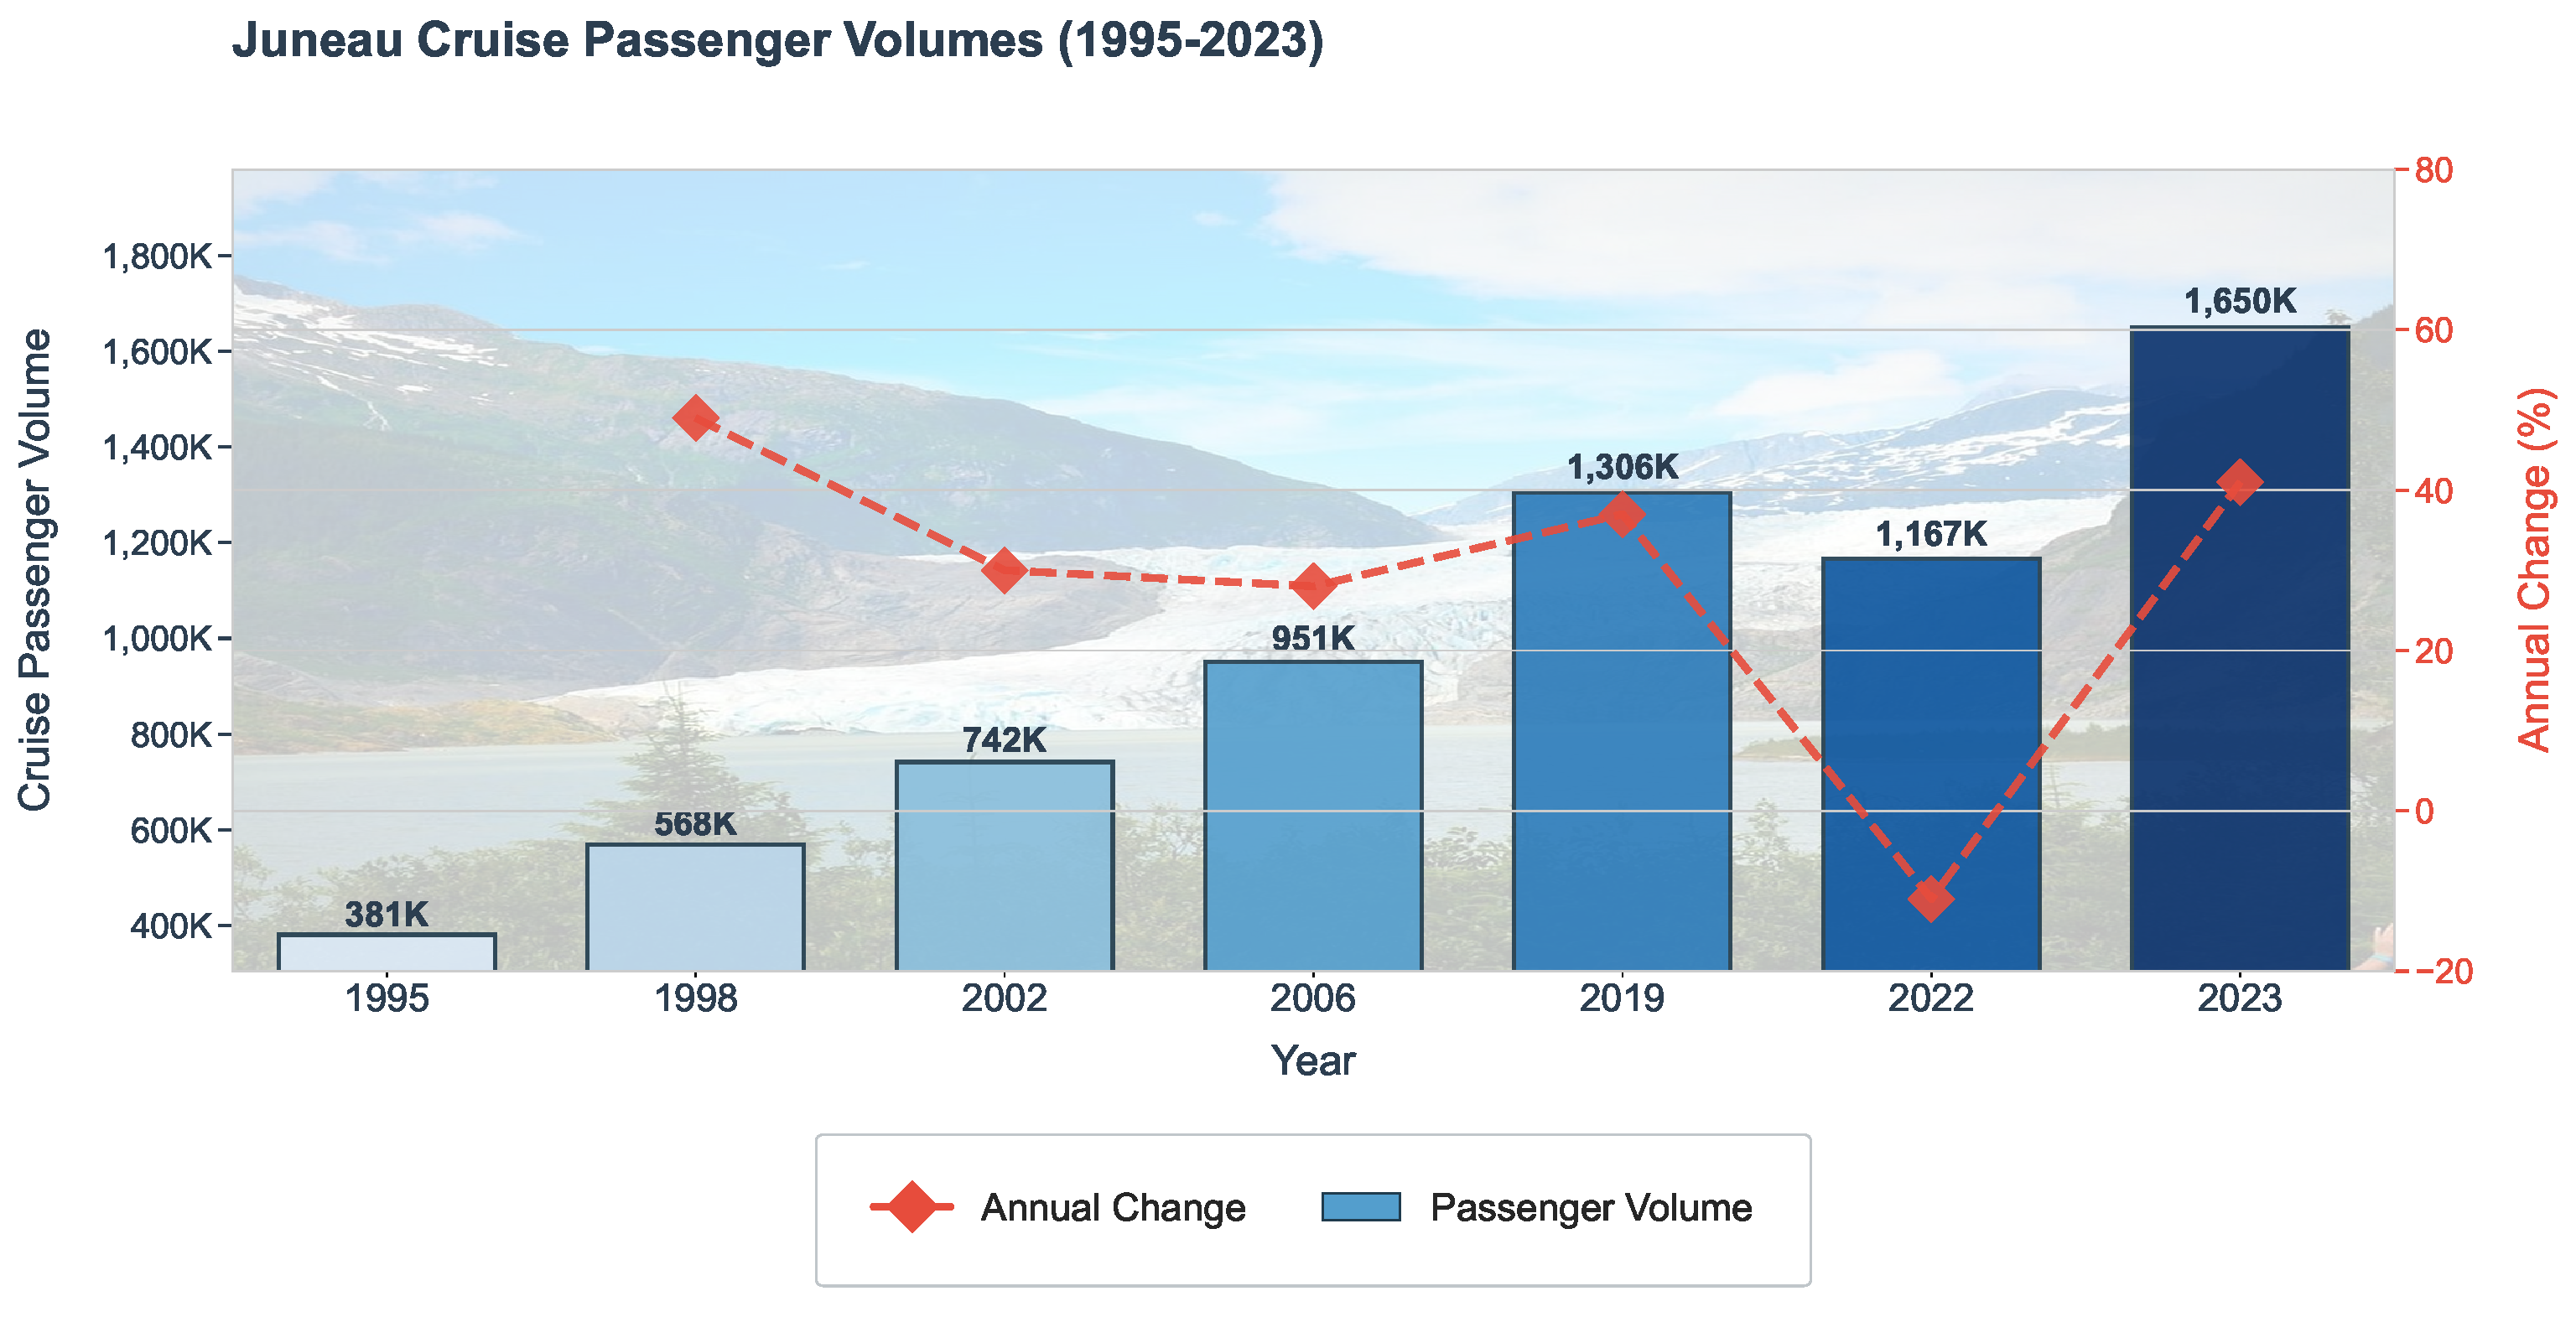
\includegraphics[width=14cm]{totaltour_1.pdf}
  \caption*{Noted: Passenger volumes in 2022 decreased due to COVID-19}\label{fig1}
  \end{figure}

  \subsection{Restatement and Analysis of the Problem}

  We aim to explore key issues in the sustainable development of tourism by constructing a 
  multi-objective optimization model. Our research tasks primarily consist of the following three 
  interrelated aspects:
\begin{itemize}
  \item \textbf{Task 1:  Tourism Sustainability Optimization Framework} This task establishes a comprehensive analytical system combining multivariate regression, input-output analysis, and multi-objective optimization to quantify tourism-environment interactions and optimize investment strategies. Based on literature research and existing survey data, we construct a multiple regression model to examine the relationships between carbon emissions, economic benefits of tourism, resident satisfaction, and tourist numbers. Building on this basis, an input-output analysis will be used to assess the investment effectiveness in these areas: environmental protection (greenhouse gases reduction) and infrastructure development. Subsequently, a multi-objective optimization model will be developed using the NSGA-III algorithm. This model will integrate the objective functions and constraints, aiming to determine the optimal tourist carrying capacity and investment allocation plan, followed by a sensitivity analysis of key parameters.
  \begin{figure}[h!] 
    \centering
    \includegraphics[width=12cm]{Work_review02.pdf}
    \caption{Tourism Sustainability Optimization Framework} \label{fig2}
  \end{figure}
  \item \textbf{Task 2: Data-driven adaptability Summary.} This task develops a dynamic clustering methodology to implement differentiated management strategies for diverse tourism destinations. A clustering analysis will be conducted to classify different types of tourist destinations, with a focus on examining the differential characteristics of core indicators such as tourist numbers, infrastructure carrying capacity, and tourism revenue. 
  Based on the classification results, a sustainable tourism development plan corresponding to the city's development status is selected from the feasible solutions, ensuring the model's adaptability and flexibility in addressing overtourism impacts at different types of destinations.
  \item \textbf{Task 3: Evidence-based memo writing.} This task translates quantitative findings into actionable governance tools for sustainable tourism management. Based on the empirical research findings, a policy recommendation memorandum will be drafted to provide scientific decision-making support for the sustainable development of Juneau's tourism industry. The memorandum will focus on the key conclusions derived from the model's empirical analysis and offer actionable policy recommendations.
  \end{itemize}
  There is a significant theoretical and practical connection between the tasks outlined above: The foundational model developed in Task 1 provides the methodological support for subsequent research; 

\section{Assumptions and Justification}
To simplify the problem and make it convenient for us to simulate real-life conditions, we
make the following basic assumptions, each of which is properly justified.
\begin{itemize}
  \item \textbf{We conceptualize glacial ablation as an environmental baseline parameter.} 
  Glacial ablation constitutes the principal constraint on regional tourism development as a long-term geomorphic process. 
  $2010-2020$ observations demonstrate sustained annual retreat ($5.9 km^3$) with 
  limited interannual variability\cite{abc}. Our passage posits glacial mass balance systems 
  function independently from tourism dynamics, quantifying their tourism impact 
  as an environmental baseline parameter.
  %\item \textbf{We assume a linear relationship between tourist numbers and tourism revenue.}
\end{itemize}
\section{List of Notation}

\begin{table}[h!]
  \centering
  \begin{tblr}{
    colspec = {X[c]X[c]}, % 自动调整列宽
    cells = {c},
    hline{1-2,9} = {-}{},
  }
  \textbf{Symbol} & \textbf{Meaning} \\
  $V_i$      & Visitor Volume      \\
  $TA^\alpha$      & Tax Allocation in area $\alpha$     \\
  $TR_i$   & Tourism Revenue      \\
  $DS_i$      & Resident Dissatisfaction       \\
  $C_i$        & Carbon Emissions      \\
  $S_i$  & Infrastructure Stress      
  \end{tblr}
  \caption{List of Notation} 
\end{table}

\section{Data Pre-processing}
Since there is no data provided in the question, we consulted relevant survey 
results and research reports. The data we found about Greenhouse Gas Emissions, Number of Tourists and Total Tourism Revenue from 2011 to 2023 are as Table \ref{tab:tourism}:
% \marginnote{Given the substantial disruptions caused by the COVID-19 pandemic to the tourism sector during 2021-2022, our passage will systematically exclude anomalous observations from this period to ensure analytical validity.}
\begin{itemize}
  \item \textbf{Comprehensive evaluation indicators of tourism industry}\par
  Given that businesses serving the tourism industry also typically cater to the 
  residents of Southeast Alaska, such as restaurants and support services for air and 
  water transportation, it is not feasible to attribute employment and wage data 
  solely to the tourism sector. In the Economic Indicators Reports published annually 
  by the City of Juneau, all positions within the leisure, hospitality, and transportation 
  sectors are aggregated to assess the overall health of the tourism industry. 
  Consequently, the total income reported for the Leisure \& Hospitality sector is 
  considered representative of the total income generated by the tourism industry.
  % ===== 颜色定义 =====
\definecolor{TableHeader}{RGB}{70,130,180}      % 表头颜色 (蓝钢色)
\definecolor{ZebraEven}{RGB}{248,248,248}       % 斑马纹背景 (浅灰)
\definecolor{ColEmission}{RGB}{225,245,255}     % 温室气体列颜色 (极浅蓝)
\definecolor{ColTourists}{RGB}{245,255,230}     % 游客数列颜色 (薄荷绿)
\definecolor{ColRevenue}{RGB}{255,245,210}      % 收入列颜色 (浅鹅黄)
\definecolor{TableLine}{RGB}{220,220,220}       % 表格线颜色
\definecolor{NoteColor}{RGB}{90,90,90}          % 注释文字颜色

\begin{table}[htbp]
  \centering
  \caption{Environmental Impact and Tourism Development (2011-2023)}
  \label{tab:tourism}
  \begin{tblr}{
    width = 0.85\linewidth,
    colspec = {lrrr},
    row{1} = {bg=TableHeader, fg=white, font=\bfseries},  % 表头样式
    row{even} = {bg=ZebraEven},                            % 斑马纹效果
    column{2} = {bg=ColEmission},                          % 第2列背景
    column{3} = {bg=ColTourists},                          % 第3列背景
    column{4} = {bg=ColRevenue},                           % 第4列背景
    hlines = {TableLine},                                  % 水平线样式
    vlines = {},                                           % 无垂直线
    cells = {font=\small},                                 % 统一字号
    cell{2-10}{2-4} = {mode=math},                         % 数学模式
  }
  % ===== 表头 =====
  \SetCell{bg=TableHeader}Year 
    & \SetCell{bg=TableHeader}Greenhouse Gas Emissions 
    & \SetCell{bg=TableHeader}Number of Tourists 
    & \SetCell{bg=TableHeader}Total Tourism Revenue \\
  
  % ===== 单位行 =====
  & (ton CO\textsubscript{2}e) 
    &  
    & (USD) \\
  
  % ===== 数据行 =====
  2011 & 71,727.76    & 1,556,800    & N/A \\
  2012 & 113,587.49   & 1,586,000    & 27,713,469 \\
  2013 & 95,652.89    & 1,693,800    & 28,374,275 \\
  2014 & 76,765.20    & 1,659,600    & 30,711,658 \\
  2015 & 51,892.62    & 1,780,000    & 75,068,464 \\
  2016 & 56,959.98    & 1,857,500    & 79,294,933 \\
  2017 & 49,644.26    & 1,926,300    & 82,318,620 \\
  2018 & 49,236.73    & 2,026,300    & 92,094,125 \\
  2019 & 104,822.60   & 2,213,000    & 103,225,389 \\
  2022 & N/A          & N/A          & 119,520,965 \\
  2023 & N/A          & N/A          & 134,631,332 
  \end{tblr}
  
  % ===== 注释 =====
  \vspace{0.5em}
  {\small\color{NoteColor}\raggedright 
    Data for 2020-2021 affected by COVID-19 are not included.
  }
\end{table}
  \item \textbf{Questionnaire survey on residents' satisfaction}\par
  We reviewed the tourism satisfaction survey data from the Juneau City Government 
  and plotted the corresponding charts. The results indicate that residents are 
  concerned about tourism-related issues.\par Most are dissatisfied with crowding and 
  sidewalk congestion, with scores between 1 and 2. Regarding overcapacity and 
  visitor limits, attitudes are neutral, with scores between 2 and 3, showing some 
  support but not universal agreement. Traffic congestion is also a concern, with 
  scores mostly between 2 and 3. Cruise frequency and emissions also raise concern, 
  as residents worry about their environmental impact. In contrast, there is strong 
  support for clean energy, with scores concentrated between 4 and 5. Flight emissions 
  also received attention, reflecting concern about the environmental impact of 
  aviation.\par Overall, residents hope tourism can drive economic growth while prioritizing 
  environmental protection. Detailed survey results are shown in Figure \ref{fig:satisfy}.
  \begin{figure}[h] 
    \centering
    {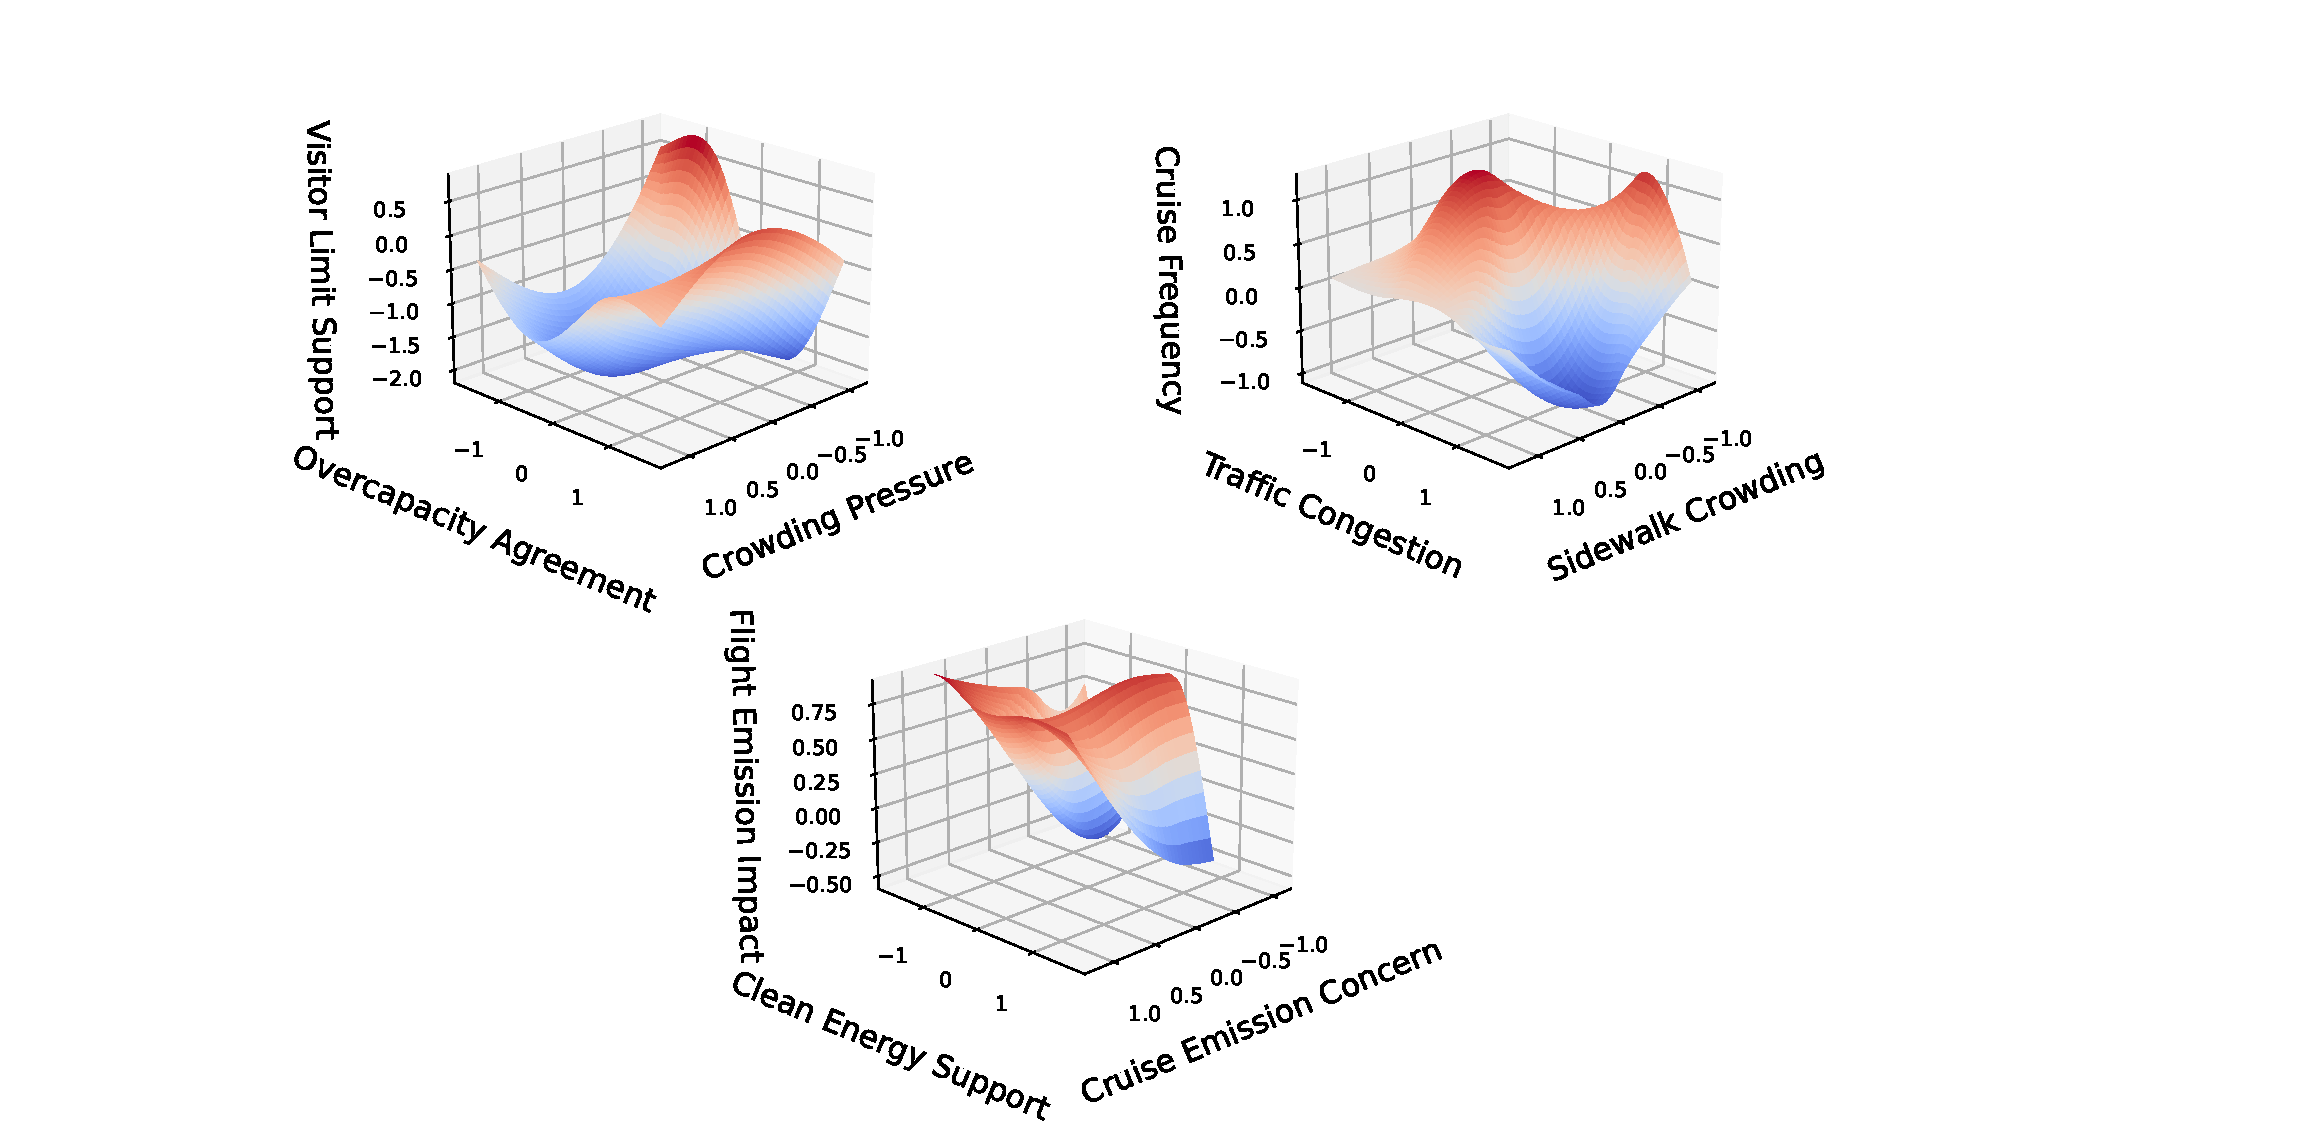
\includegraphics[width=12cm]{Satisfaction Questionnaire.pdf}} % 减小宽度留出边框空间
    \caption{Result of Satisfaction Questionnaire} \label{fig:satisfy}
  \end{figure}
  \item \textbf{Tax income}\par
  We know from the local regulations of Juneau that the local government imposes 9\% Hotel/Motel Tax and 5\% Sales Tax on tourists, with a total tax rate of 14\%. From this, we can conclude that the relationship between local taxes and tourist consumption, that is, local economic income, is:
  \begin{equation}
    \label{eq:tax}
    TA^\alpha = 0.14 \times TR_i
  \end{equation}
  where $TA$ is the total tax income and $TR$ is the total tourism revenue.
  \item \textbf{Calculate the total number of visitors}\par
  Given the missing data on total tourist numbers for certain years and the significant positive correlation between cruise tourist numbers and total tourist volume, we incorporated the total tourist volume and cruise tourist numbers from 2011 to 2019 into the following regression equation:

\begin{equation}
  \label{eq:totalvisitor}
C_i = \beta_0 + \beta_1 \cdot C_i^{\text{cruise}} + \epsilon
\end{equation}

The parameter estimation yielded:  
\(\beta_0 = 166\,878.151\), \(\beta_1 = 1.572\)
\item \textbf{Limitation of total number of tourists}\par
According to the terms of the agreement announced by the city, beginning in 2026, a daily passenger capacity limit of 16,000 will be enforced from Sunday to Friday, while Saturdays will be restricted to 12,000 passengers.  
Combined with the city of Juneau's 200 navigable days per year for cruise ships, these constraints yield a maximum annual cruise passenger volume of approximately 2,628,600 passengers/year under this policy. Based on \eqref{eq:totalvisitor}, the annual maximum tourist capacity is calculated as 4,299,037 passengers/year.
  \item \textbf{Calculation of Daily Visitor Distribution}\par
  Based on the annual total of 1,638,902 cruise visitors in Juneau City Port in 2023 and the recorded days exceeding daily visitor thresholds (Table \ref{tab:threshold}), we assume the daily visitor count
  \begin{table}[h!]
    \centering
    \rowcolors{2}{gray!10}{white} % 斑马纹:偶数行浅灰填充,奇数行白色
    \begin{tabular}{cc}
      \toprule
      \rowcolor{gray!20} % 单独设置表头背景色
      \textbf{Daily Visitor Threshold (visitors/day)} & \textbf{Days Exceeding Threshold (days)} \\
      \midrule
      5,000  & 40 \\
      6,000  & 40 \\
      7,000  & 39 \\
      8,000  & 37 \\
      9,000  & 30 \\
      10,000 & 25 \\
      11,000 & 22 \\
      12,000 & 15 \\
      13,000 & 13 \\
      14,000 & 9  \\
      15,000 & 6  \\
      16,000 & 4  \\
      17,000 & 3  \\
      18,000 & 2  \\
      19,000 & 1  \\
      \bottomrule
    \end{tabular}
    \caption{Daily Visitor Thresholds and Exceedance Days in 2023}
    \label{tab:threshold} % label移至caption后以符合交叉引用规范
\end{table}

  $V^{daily}$ follows a normal distribution $\mathcal{N}(\mu, \sigma^2)$. The probability distribution fitting proceeds as follows:
  $$\mu = \frac{1{,}638{,}902}{365} \approx 4{,}490.1 \, \text{visitors/day}$$
  The daily average visitor count is derived from the annual total.\\
  For each visitor threshold $v^{daily}_i$, its cumulative probability is computed as:
  $$P(V^{daily} \leq v^{daily}_i) = \frac{365 - D_i}{365}$$
  where $D_i$ denotes the number of days exceeding $v^{daily}_i$. The corresponding standard normal quantile is obtained using the inverse cumulative distribution function:
  $$Z_i = \Phi^{-1} \left( P(V^{daily} \leq v^{daily}_i) \right)$$
  A regression relationship between the standardized variable and visitor count is established:
  $$v^{daily}_i - \mu = \sigma Z_i + \epsilon$$
  An intercept-free regression model is employed for fitting, yielding an estimated standard deviation $\sigma = 4589.3$ in Figure \ref{fig:dailyvisitor}.\par
  \begin{figure}
    \centering
    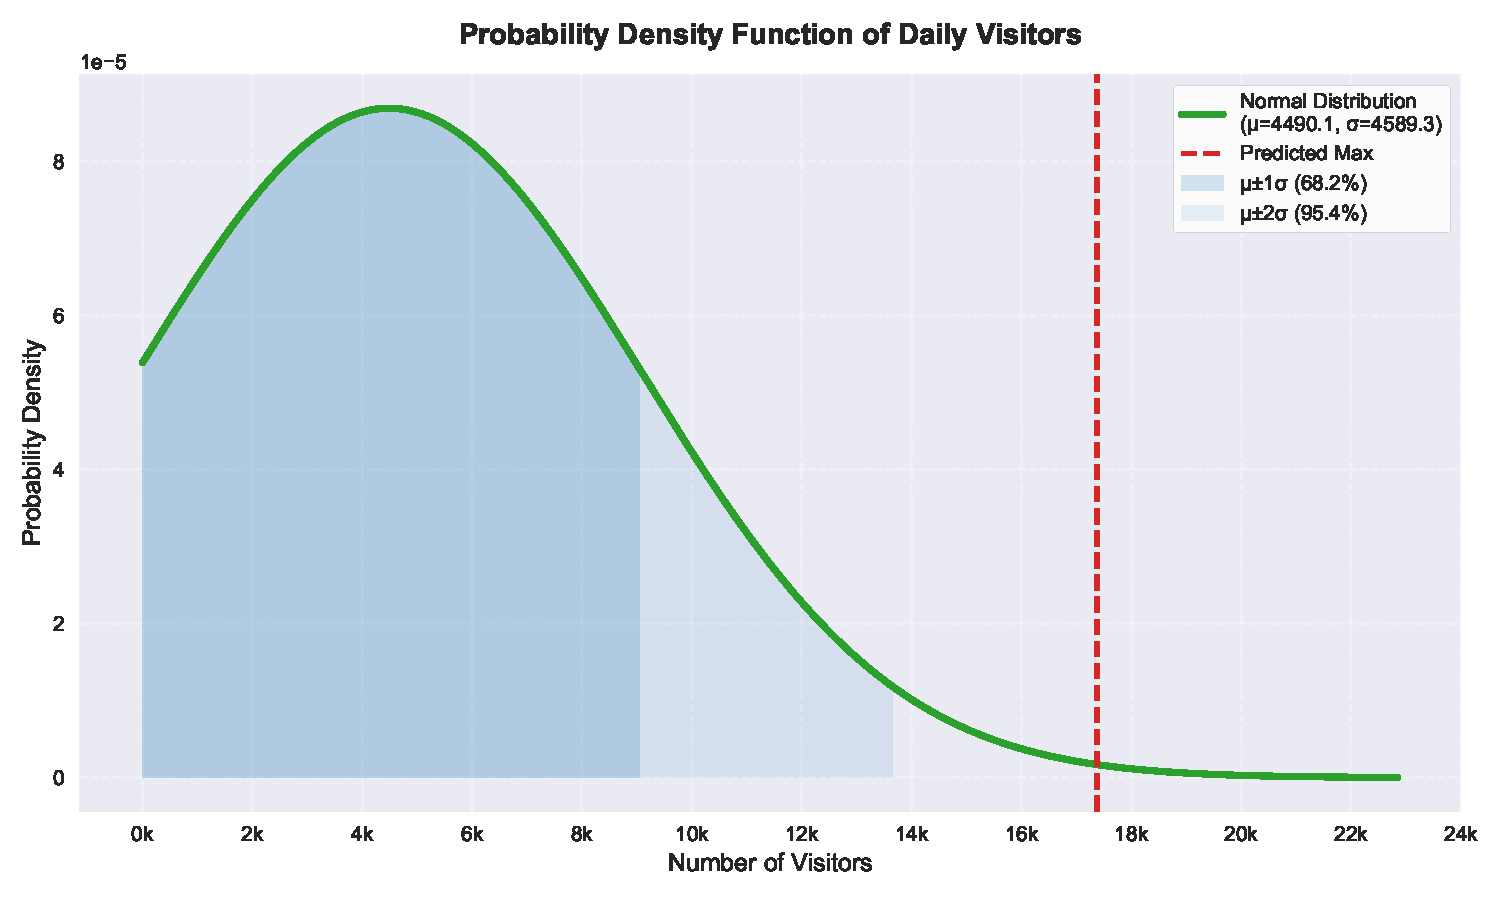
\includegraphics[width=15cm]{dailyvisitor.pdf}
    \caption{Daily Visitor Distribution in Juneau City} \label{fig:dailyvisitor}
  \end{figure}
  In summary, the daily tourist volume in Juneau City approximately follows a normal distribution 
  \begin{equation}
    \label{eq:dailyvisitor}
    \mathcal{N}(\mu, (4589.3)^2)
  \end{equation}
  
  
\end{itemize}

\section{Task1: Tourism Sustainability Optimization Framework}
\subsection{Precondition description}
\subsubsection{Relationship between Carbon Emissions and Tourist Numbers}
We selected greenhouse gas emission data from 2011 to 2019 as the dependent variable to examine the dynamic impacts of tourist numbers and temporal factors on emissions. The independent variables were chosen based on the following rationale:
\begin{itemize}
  \item \textbf{Quadratic term of tourist numbers:} Reflects the nonlinear relationship between tourism activities and emissions, capturing changes in marginal effects.
  \item \textbf{Year deviation term ($Year-2011$):} Quantifies cumulative effects of environmental policy implementation while eliminating baseline year selection bias.
  \item \textbf{Data standardization:} Tourist numbers were converted to millions ($V_i^M$) to enhance model stability.
\end{itemize}
Based on this analysis, we established a quadratic regression model with temporal trend:
\begin{equation}
  C_i = \beta_0 + \beta_1 (\text{Year-2011}) + \beta_2 V_i^M + \beta_3 \left( V_i^M \right)^2 + \epsilon 
\end{equation}
\textbf{Through solving the equation, we derived results as shown in the Figure \ref{fig:carbon}}
\begin{figure}[h!]
  \centering
  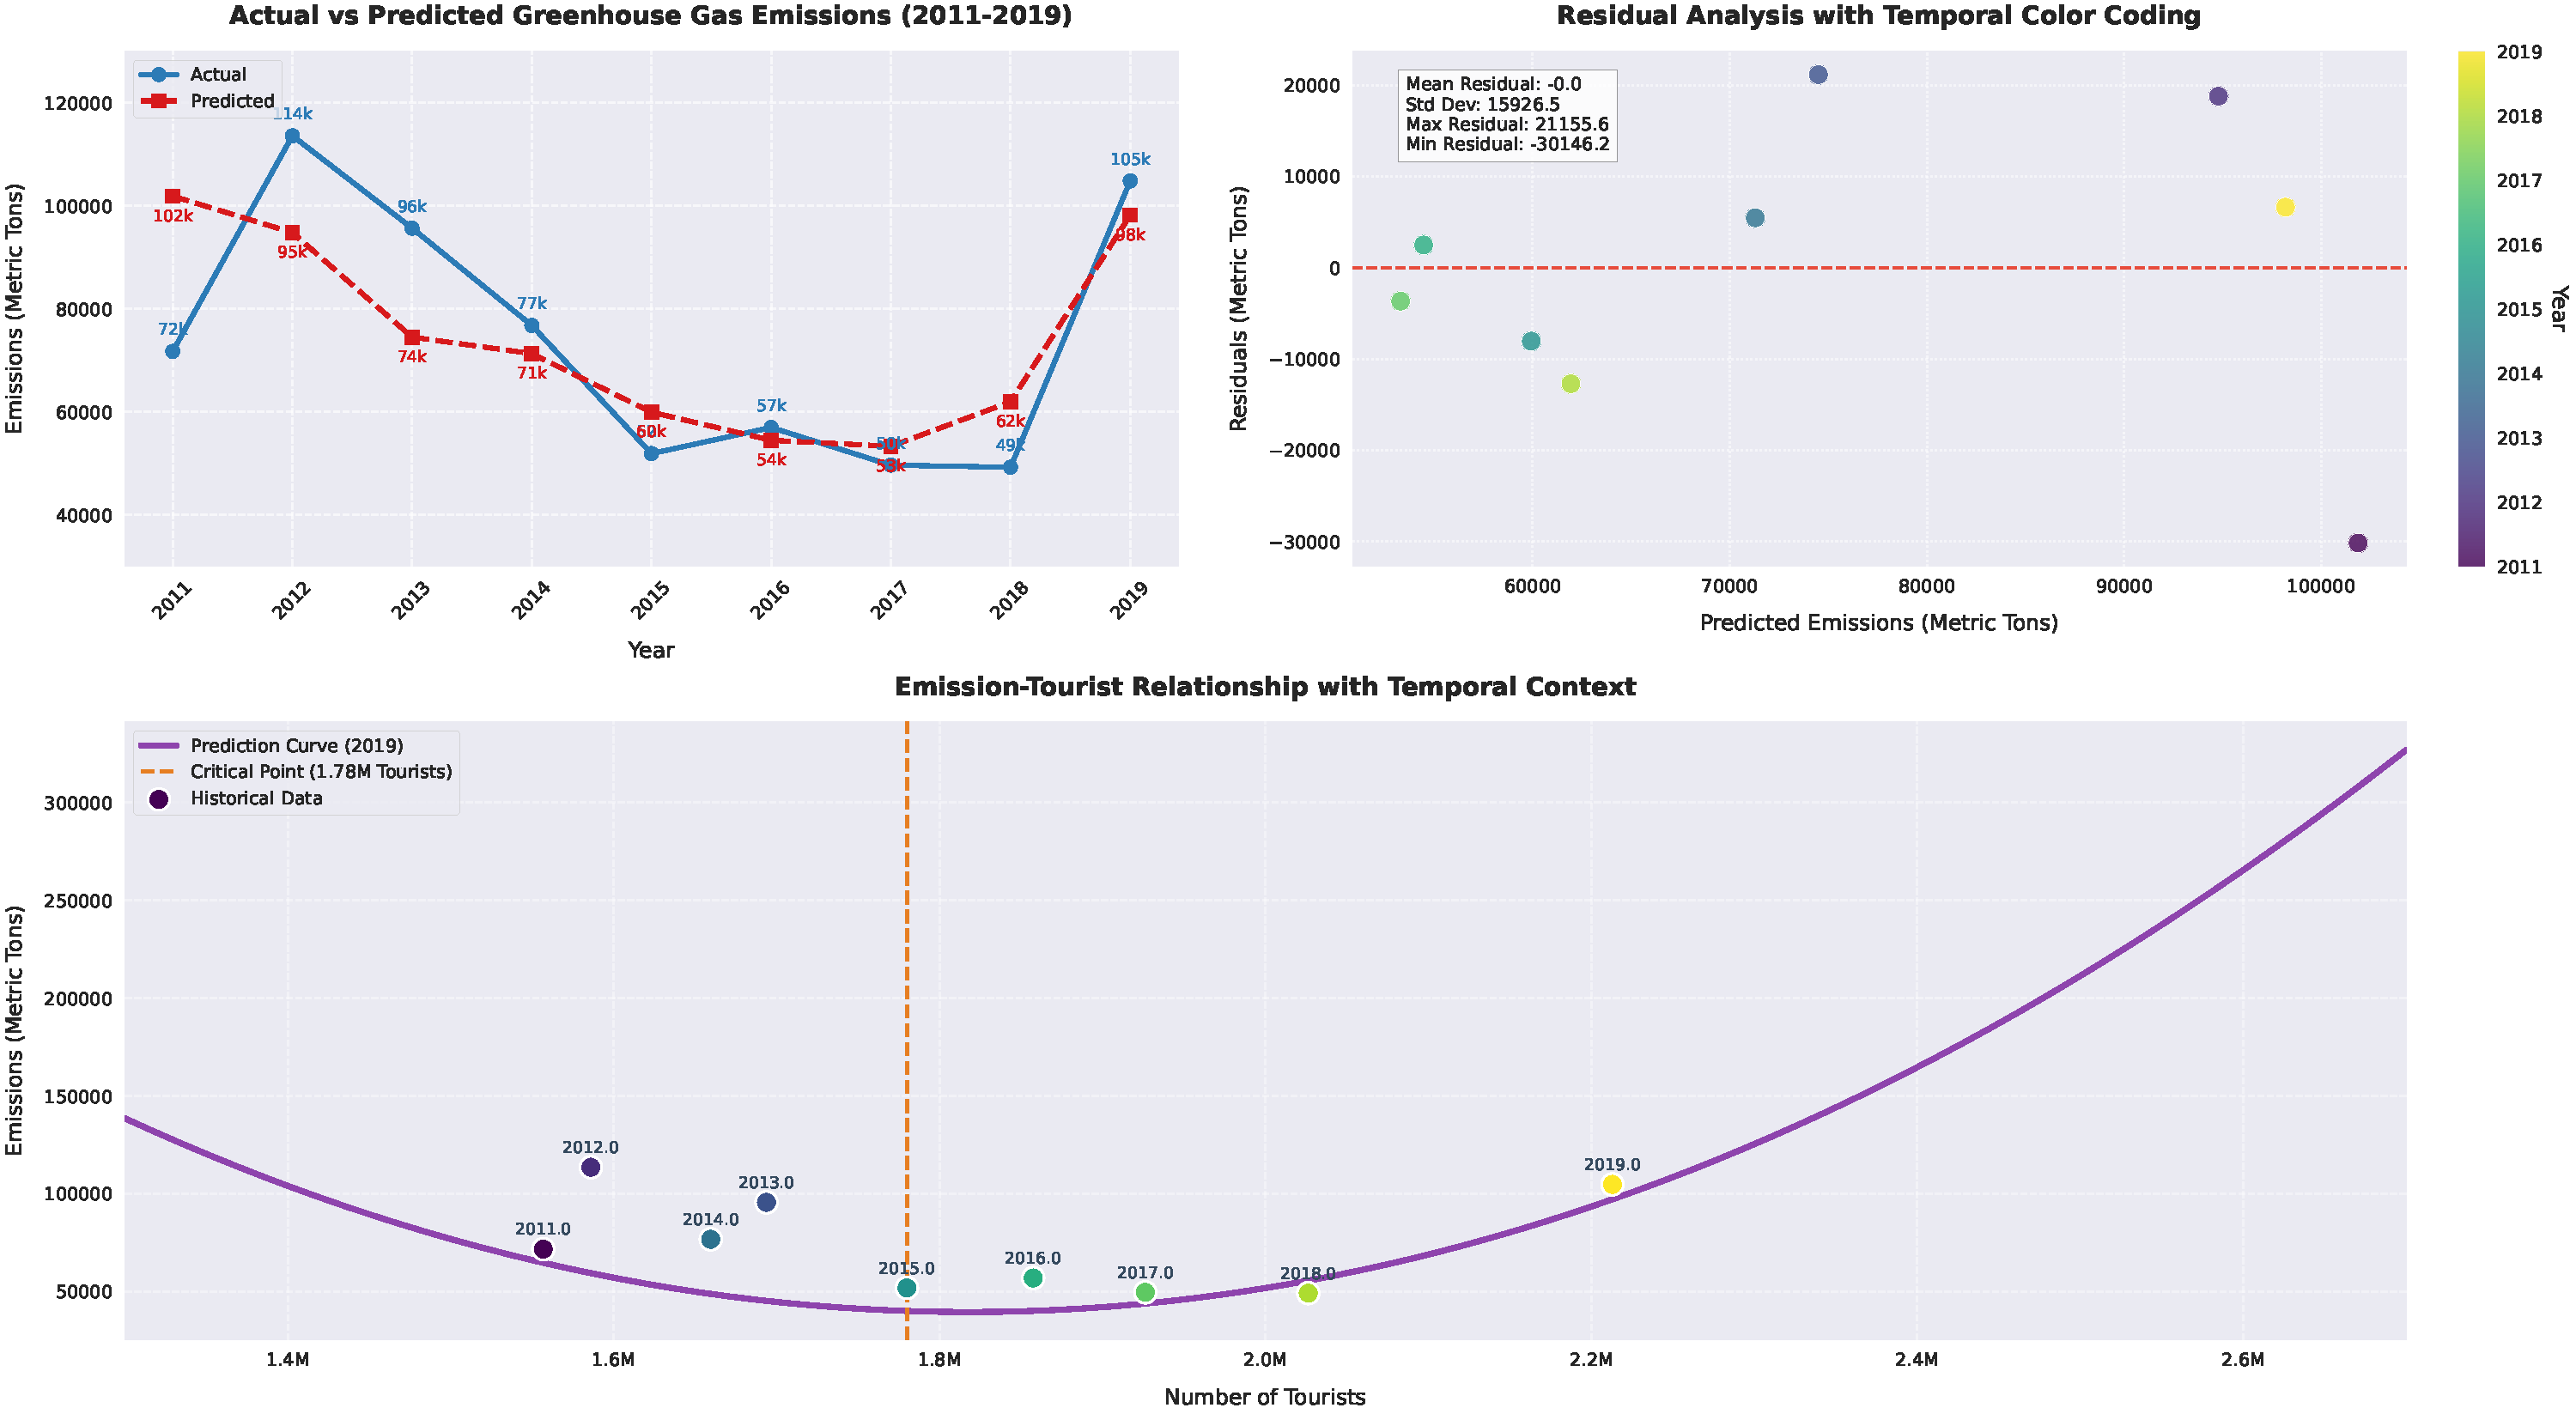
\includegraphics[width=16cm]{tournum-carbon.pdf}
  \caption{Relationship between Carbon Emissions and Tourist Numbers}  % 添加标题
  \label{fig:carbon}                   % 标签放在caption之后
\end{figure}
\begin{itemize}
  \item $\beta_0 = 1,151,001$ represents the baseline intercept for the reference year.
  \item $\beta_1 = -6,723$ quantifies the annual emission reduction effect (unit: metric tons per year).
  \item $\beta_2 = -1,198,962$ and $\beta_3 = 337,702$ jointly capture the nonlinear effects of tourism activities on carbon emissions.
\end{itemize}
\textbf{By deriving the first derivative of this function:}
\begin{equation}
  \frac{\partial C}{\partial V} = \beta_2 + 2\beta_3 V = 0 \quad \Rightarrow \quad V_c = -\frac{\beta_2}{2\beta_3}
\end{equation}
Substituting estimated parameters yields:
\begin{equation}
  V_c = \frac{1,198,962}{2 \times 337,702} \approx 1.78 \text{ million}
\end{equation}
This demonstrates that when Juneau's tourist numbers exceed 1.78 million visitors per year, subsequent growth in tourism will lead to a significant increase in local $CO_2$ emissions, causing environmental degradation through accelerated glacier melting and other ecological consequences.
\subsubsection{Tourism revenue regression model}
We employed regression analysis to investigate the quantitative relationship between tourist volume and tourism revenue. The linear regression model constructed based on the least squares method is as follows:
\begin{equation}
  TR_i = \beta_0 + \beta_1 V_i + \epsilon
\end{equation}
\textbf{Through regression analysis, the following empirical results were obtained}
\begin{itemize}
  \item \textbf{The regression coefficient $(\beta_1 = 136.581)$}  indicates that for each additional tourist, tourism revenue increases by an average of $\$136.581$. This coefficient quantifies the direct marginal effect of tourist numbers on tourism revenue.
  
  \item \textbf{The intercept term $(\beta_0 = -186,843,122)$} suggests that when tourist numbers equal zero, the predicted tourism revenue would be $\$-186,843,122$, reflecting fixed costs and other unobserved factors affecting the tourism industry in Juneau.
  
  \item \textbf{The coefficient of determination $(R^2 = 0.844)$} demonstrates that the model explains $84.4\%$ of the variance in tourism revenue, indicating a strong goodness-of-fit to the observed data.
  
  \item Statistical significance tests reveal that the regression coefficient exhibits a \textbf{t-statistic of $5.701$} with a corresponding \textbf{p-value of $0.001$}, which is statistically significant at the $\alpha = 0.05$ level. These results confirm a significant linear relationship between tourist numbers and tourism revenue, rejecting the null hypothesis of no association. 
\end{itemize}
\subsubsection{Structural equation model of residents' satisfaction}
Through Structural Equation Modeling (SEM), this study systematically investigates the complex relationships among tourist volume, carbon emissions, glacier status, and satisfaction as Figure \ref{fig:sem}.\\ 
\textbf{The model comprises four latent variables with corresponding observed indicators:}
\begin{itemize}
  \item \textbf{Tourist:} Measured by $Tourist_{Q1}$ (traffic congestion level) and $Tourist_{Q2}$ (cruise frequency), reflecting tourism activity intensity. 
  \item \textbf{Glacier (glacial status):} Evaluated through $Glacier_{Q1}$ (residents' concern about tourism-induced glacial degradation), representing glacial environment protection awareness.
  \item \textbf{Carbon (carbon emissions): } Assessed by $Carbon_{Q1}$ (residents' concern about tourism-related carbon emissions), measuring carbon emission cognition and behavioral patterns.
  \item \textbf{Satisfaction:} Integrated with $Satisfy_{Q1}$ (resident satisfaction), reflecting the interaction between environmental policies and public satisfaction.
\end{itemize}
\textbf{Significance Analysis of Critical Pathways:}\par
The model results demonstrate a statistically significant positive impact of tourist volume on satisfaction (path coefficient: $0.524$, $p < 0.05$). This suggests that increased tourist numbers may enhance overall resident/visitor satisfaction through stimulating local economic vitality or improving infrastructure investment.\par
A significant feedback effect emerges from satisfaction to glacial status (path coefficient: $0.587$,$ **p < 0.01$), indicating that heightened satisfaction may drive stricter glacial protection policies (e.g., tourist capacity restrictions), thereby alleviating glacial pressure.\par
Notably, while the negative impact of carbon emissions on satisfaction lacks statistical significance (path coefficient: $-0.204$, $p > 0.05$), its directional tendency implies potential indirect erosion of public satisfaction through environmental quality deterioration.\par
\textbf{Comprehensive Analysis:}\par
The integrated findings reveal a U-shaped correlation between tourist volume and resident satisfaction. Short-term tourism growth enhances satisfaction through economic benefits, whereas excessive long-term tourism may reduce satisfaction through \textbf{Intensified greenhouse gas emissions} and \textbf{Infrastructure pressure} \par
\begin{figure}[h!] 
  \centering
  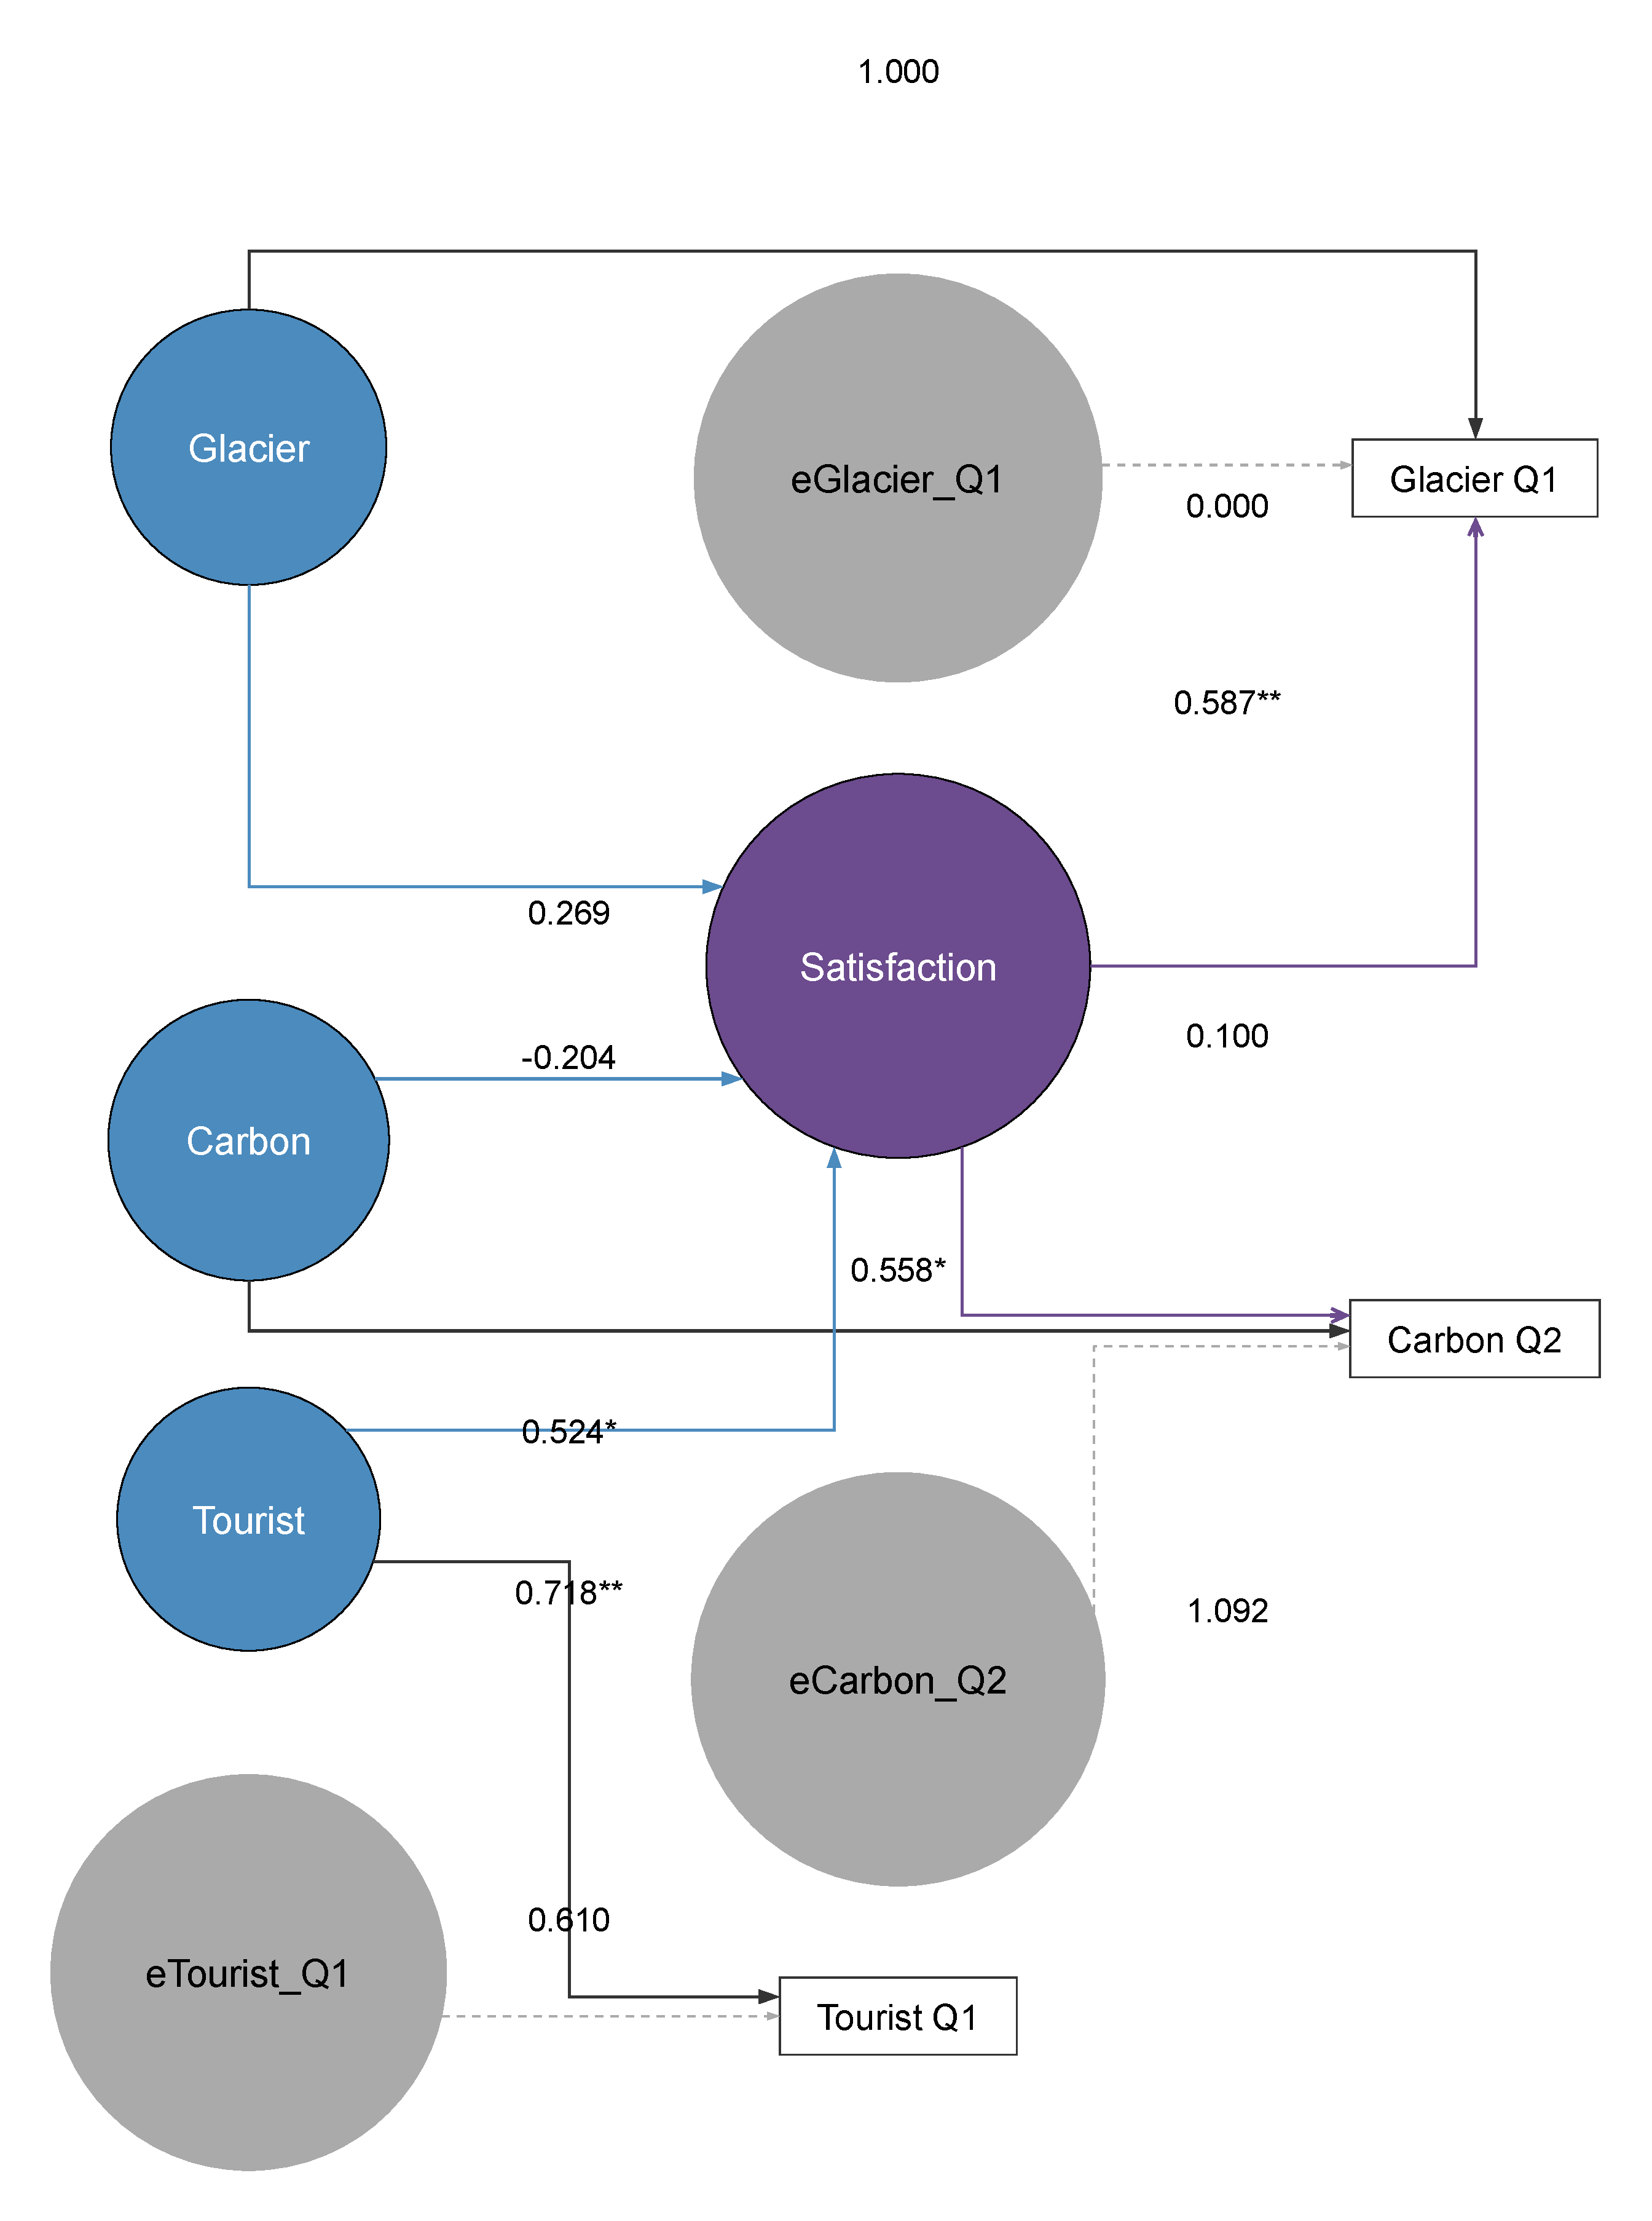
\includegraphics[width=12cm]{sem_diagram_final.pdf}
  \caption{SEM for Resident Satisfaction Surveys} \label{fig:sem}
\end{figure}
All in all,we get the following conclusions:
\begin{equation}
  DS_i = 76.62 - 0.574 V_i^M + 0.0129 \left( V_i^M \right)^2
\end{equation}
\subsubsection{Infrastructure Stress Analysis}
As the majority of tourists visiting Juneau City opt for maritime transportation, the substantial influx of visitors imposes significant strain on the port facilities and adjacent public transportation infrastructure. Based on the 2023 survey report, our analysis indicates that the maximum daily capacity of the port’s traffic system is approximately 14,000 individuals per day. Exceeding this threshold would result in substantial tourist overcrowding. Consequently, we define the transportation infrastructure capacity limit of Juneau City as the condition under which tourist volume remains below this maximum capacity for no more than 97.5\% of days annually. The daily tourist volume is approximated to follow a normal distribution throughout the year as \eqref{eq:dailyvisitor}.\par  
\subsubsection{Input-output of additional expenditure by sector}
We collected relevant information to determine the input-output of additional spending in different areas to determine our additional spending plan.
\begin{itemize}
  \item \textbf{Input-output in the field of carbon emission reduction:} We have examined an environmental justice initiative entitled the Alaska Carbon Reduction Fund, implemented by Renewable Juneau, a non-profit organization based in Juneau. This project allocates funds to replace oil-fired heating systems with high-efficiency, emission-free air-source heat pumps in low-income households. According to disclosed data from the organization, the carbon abatement cost of this initiative amounts to $\$46$ per metric ton of carbon dioxide equivalent $(CO_2e)$ reduced. This metric has been utilized for input-output calculations in the field of carbon emission reduction.
  \item \textbf{Input-output in infrastructure construction:} Based on previous analyses indicating that the substantial tourist influx during peak seasons exerts considerable pressure on Juneau's public transportation system, this study conducts a cost-benefit analysis of infrastructure investments from the perspective of public transportation input-output efficiency.\par
  According to statistical data from the American Public Transportation Association (APTA), the average operational cost of public transit systems in the United States ranges between USD 3-5 per passenger trip. Assuming Juneau's operational costs approximate the national average, with fare revenue covering approximately 50\% of operational expenditures, our calculations demonstrate that each additional passenger served by the transit system would require an incremental investment of USD 200. This derived value results from the differential between total operational costs and fare recovery rates.
\end{itemize} 

\subsection{Model construction and algorithm implementation}
\subsubsection{Multi-objective optimization model construction}
\textbf{Define the 2-dimensional decision variable \( \mathbf{x} = [V_i, TA_{\alpha}] \), where:}
\begin{itemize}
    \item \( V_i \): Annual tourist volume (people/year), range \([0, 4.299 \times 10^6]\)
    \item \( TA_{\alpha} \): Environmental tax allocation ratio (\%), range \([0, 100\%]\)
\end{itemize}

\textbf{Define the objective functions:}
\[
\max \, f_1 = -TR_i = \beta_0 - \beta_1 V_i
\]
\[
\min \, f_2 = C_i = \beta_2 - \beta_3 - \beta_4 V_i + \beta_5 V_i^2 - \frac{TR_i \cdot \beta_6 TA_{\alpha}}{\beta_7}
\]

\textbf{Subject to constraints:}
\[
\begin{cases} 
    g_1 = V_i - \beta_0^1 \leq 0, \\ 
    g_2 = \dfrac{V_i^{\text{cruise}}}{\beta_0^2} + \beta_{1}^2 - S_i \leq 0, \\
    g_3 = \big( \beta_{0}^3 - \beta_{1}^3 V_i + \beta_{2}^3 V_i^2 \big) - \beta_{3}^3 \leq 0,
\end{cases}
\]
\subsubsection{Algorithm selection and parameter setting}
We used the \textbf{NSGA-III algorithm} to solve the optimization problem. The algorithm uses a non-dominated sorting genetic algorithm based on reference points. By systematically generating reference directions, it guides the population to evenly distribute in the target space, avoids the solution set from gathering in local areas, and maintains the diversity and convergence of 
the solution set. 
%Key parameter configurations are shown in Table \ref{tab:params}.
  % For table caption styling
% \begin{table}[!ht]
% \centering
% \caption{Key Parameter Configuration}
% \label{tab:params}

% \begin{tabular}{@{}lll@{}}
% \toprule
% \textbf{Parameter} & \textbf{Value/Method} & \textbf{Theoretical Basis} \\
% \midrule
% Reference Direction Generation Strategy & Das-Dennis Method & Ensure uniform coverage \\
% Number of Reference Directions & 12 & Balance computational efficiency \\
% Population Size & 100 & avoiding premature convergence \\
% Termination Condition & 300 generations & curve indicating steady state \\
% \bottomrule
% \end{tabular}
% \label{tab:params}
% \end{table}
\subsection{Optimization results analysis}
\begin{table}[htbp]
  \centering
  \caption{All Feasible Solutions with Environmental and Economic Indicators}
  \label{tab:solutions}
  \sisetup{
    group-separator = {,},  % 千位分隔符
    table-number-alignment = center,
  }
  \begin{tabular}{
    l  % 新增序号列(左对齐)
    S[table-format=7.0]  % 游客量
    S[table-format=2.2]  % 税收占比
    S[table-format=3.2]  % 经济收益
    S[table-format=6.2]  % 碳排放
  }
  \toprule
  {\textbf{No.}} &  % 新增序号列标题
  {\textbf{Visitor Volume}} & 
  {\textbf{$TA^{environment}$ (\%)}} & 
  {\textbf{Total Revenue (million)}} & 
  {\textbf{Carbon Emissions}} \\
  \midrule
  1  & 2256779 & 50.78 & 121.39 &  52261.30 \\  % 添加序号
  2  & 2530518 & 61.40 & 158.78 & 155696.77 \\
  3  & 2612080 & 56.06 & 169.92 & 200233.36 \\
  4  & 2392205 & 70.76 & 139.89 &  91139.11 \\
  5  & 2556476 & 59.44 & 162.32 & 169469.73 \\
  6  & 2359848 & 71.67 & 135.47 &  78586.32 \\
  7  & 2640759 & 54.34 & 173.83 & 216959.49 \\
  8  & 2449582 & 66.88 & 147.72 & 116217.75 \\
  9  & 2328394 & 76.06 & 131.17 &  65681.00 \\
  10 & 2477035 & 64.55 & 151.47 & 129288.21 \\
  11 & 2503671 & 63.05 & 155.11 & 142148.55 \\  % 原数据中此行游客量应为2503671(原文误为2593671)
  12 & 2584167 & 57.35 & 166.10 & 184714.19 \\
  13 & 2421627 & 68.89 & 143.91 & 103644.60 \\
  \bottomrule
  \end{tabular}
\end{table}
\begin{figure}
  \centering
  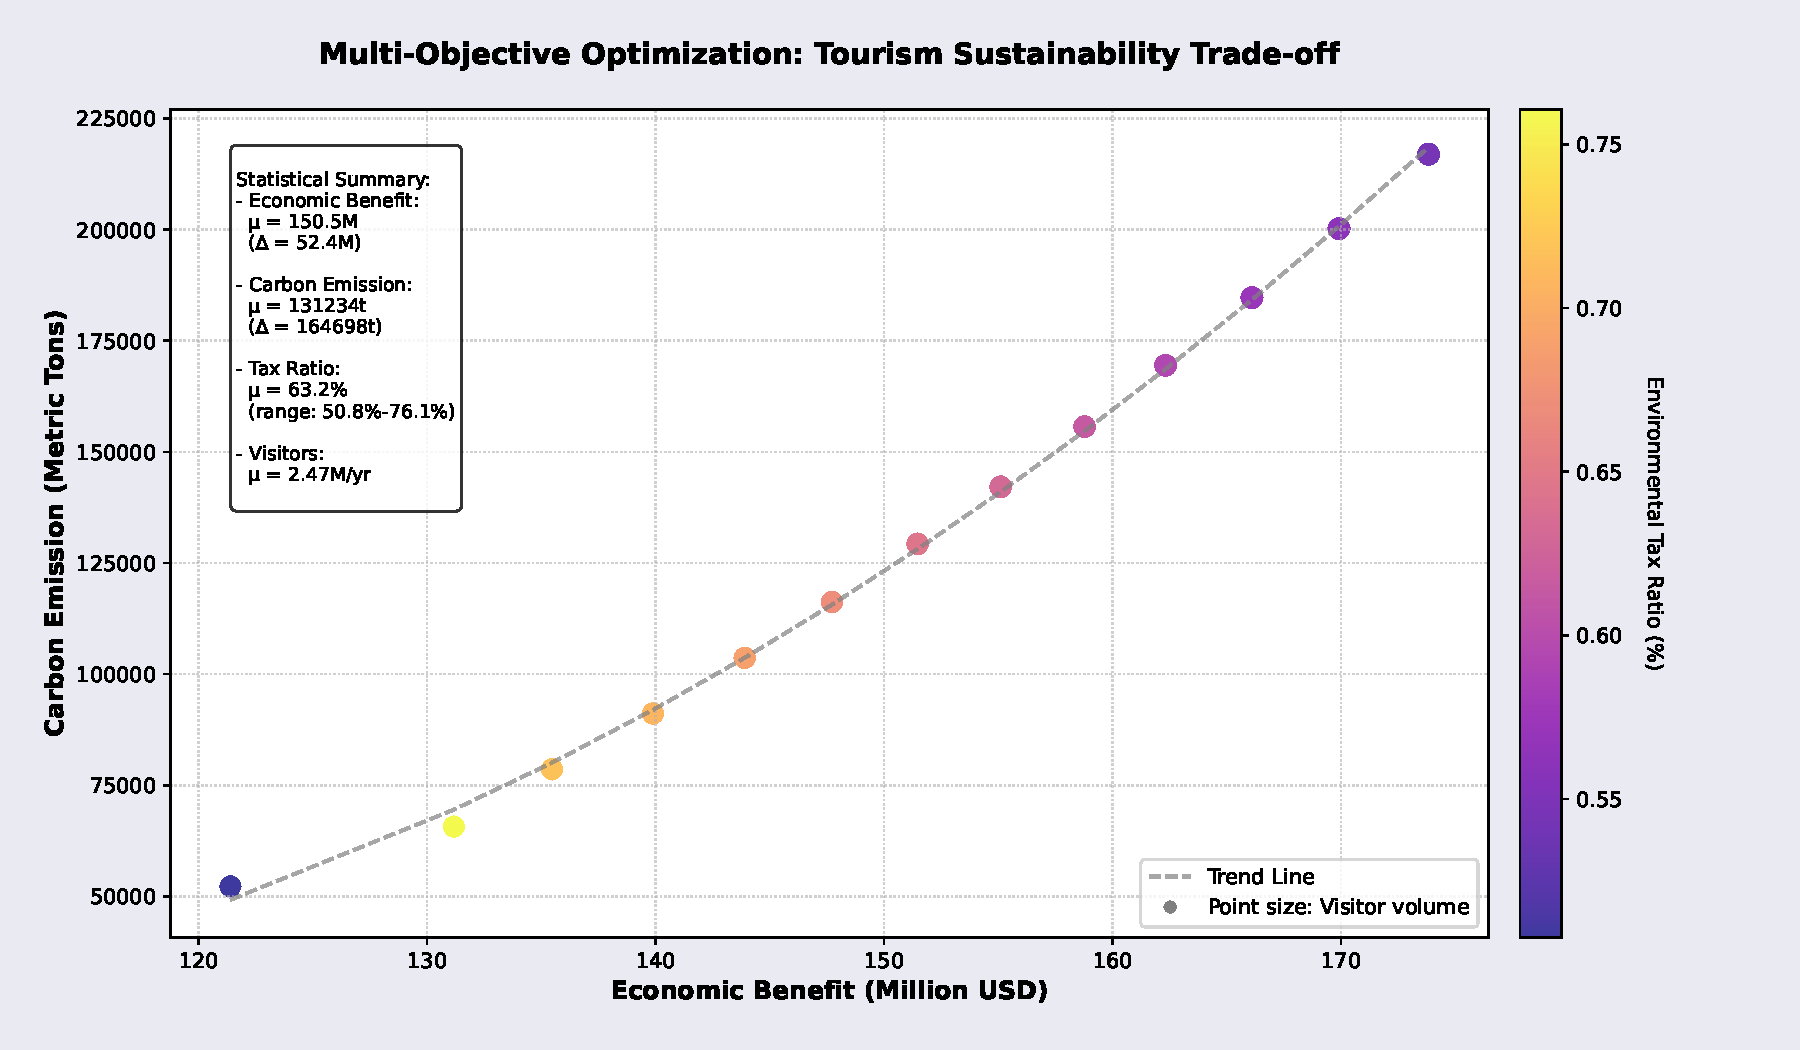
\includegraphics[width=16cm]{NSGA_3_final.pdf}
  \caption{NSGA-III Algorithm Flowchart} \label{fig:nsga}
\end{figure}
Through a comprehensive analysis of 13 sets of feasible solutions (Table \ref{tab:solutions}), significant trade-offs emerge among the indicators of tourist volume, environmental protection expenditure ratio, economic returns, and greenhouse gas emissions across different schemes. From the perspective of economic return maximization, Scheme 7 (2,640,800 annual visitors) achieves the highest economic returns of 173.83 million dollar, but simultaneously exhibits the largest environmental cost with greenhouse gas emissions reaching 216,959.49 tonnes. Scheme 9 (2,328,400 annual visitors) demonstrates optimal sustainability characteristics, featuring the lowest greenhouse gas emissions (65,681.00 tonnes) and the highest environmental protection expenditure ratio (76.06\%), albeit with notably inferior economic returns of 131.17 million dollar.

Notably, Scheme 4 (2,392,200 annual visitors) achieves superior comprehensive benefits: maintaining relatively high economic returns (139.89 million dollar) and environmental protection expenditure ratio (70.76\%) while reducing greenhouse gas emissions (91,139.11 tonnes) to approximately 30\% below the average level. Calculated by carbon emission intensity per unit economic return, this scheme achieves 651.7 tonnes/million dollar, significantly outperforming Scheme 7's 1,248.1 tonnes/million dollar, indicating higher resource utilization efficiency. Additionally, Scheme 6 (2,359,800 annual visitors) demonstrates effective balance between emission control (78,586.32 tonnes) and economic returns (135.47 million dollar), with its environmental protection expenditure ratio reaching 71.67\%, demonstrating sustainable development potential.

In conclusion, Scheme 7 could serve as a short-term strategy prioritizing economic growth. For sustainable development objectives, Schemes 9 and 6 present higher implementation value. For decision-makers pursuing comprehensive benefit maximization, Scheme 4 achieves Pareto improvement by balancing environmental, economic, and fiscal objectives, making it the preferred option.

Considering that Juneau's glacier tourism constitutes a nature-based destination where greenhouse gas emissions accelerate glacial retreat, we recommend adopting Scheme 6 or 9 as tourism development plans. These schemes prioritize environmental protection while maintaining economic balance, thereby achieving green development and sustainable growth.

\begin{table}[htbp]
\centering
\caption{Parameter Comparison of Alternative Schemes}
\label{tab:params}
\begin{tabular}{@{}lcccc@{}}
\toprule
Scheme & Annual Visitors (M) & $TA^{environment}$ (\%) & Total Revenue (million \$) & Emissions (10kt) \\
\midrule
6 & 2.3598 & 71.67 & 135.47 & 7.86 \\
9 & 2.3284 & 76.06 & 131.17 & 6.57 \\
\bottomrule
\end{tabular}
\end{table}


\subsection{Sensitivity analysis}
To evaluate the model robustness and analyze the impact of key parameters on the results, this study conducted a sensitivity analysis on three parameters: tourist capacity, environmental tax rate, and satisfaction threshold. The analysis results demonstrate that the model exhibits robust stability under parameter variations, with the variations of all indicators remaining within acceptable ranges.
\subsubsection{Parameter Impact Analysis}
By comparing the original results with those from the sensitivity analysis, the following variations were observed:
\begin{itemize}
  \item \textbf{Economic benefits:} The mean value remained stable at 425.6M, with fluctuation range narrowing from 352.4M to 498.7M, indicating high stability of economic benefits under parameter variations.
  \item \textbf{Carbon emissions:} The mean value slightly increased to 47,235t (approximately 13.8\% growth), with fluctuation range shifting from 41,876t to 54,328t, demonstrating strong robustness of carbon emission control policies.
  \item \textbf{Tax ratio:} The mean value maintained at 75.3\%, with stable fluctuation range between 52.4\% and 87.6\%, reflecting favorable adaptability and stability of tax policies.
  \item \textbf{Tourist volume:} The average annual number of tourists remained at 2.758M/yr, and the average daily number of tourists was about 7556, indicating that the tourist management strategy is sustainable.
\end{itemize}
\subsubsection{Sensitivity Analysis Methodology}
The sensitivity analysis employed a stratified sampling strategy:
\begin{itemize}
  \item Moderate interval (tourist capacity: 26,000–28,000, tax rate: 70\%–85\%, satisfaction threshold: 13–17) was sampled with 20 points to precisely capture subtle variations within this range.
  \item High-low intervals (i.e., boundary intervals) representing extreme scenarios were sampled with 15 points to balance computational efficiency and analytical quality.
\end{itemize}
This approach ensured precise analysis of critical parameter ranges while optimizing the allocation of computational resources, thereby enhancing the practical applicability of the sensitivity analysis.
\subsubsection{Differences from the Original Model}
\begin{itemize}
  \item \textbf{Tourist capacity constraint:} The original model is 4,299,037 persons/year, while the sensitivity analysis adjusted it to 2,500,000–3,000,000 persons/year.
  \item \textbf{Tax rate constraint:} The original model used a range of 0–1 (0–100\%), whereas the sensitivity analysis narrowed it to 0.5–1 (50–100\%).
  \item \textbf{Satisfaction threshold:} The original model employed a fixed value 15, while the sensitivity analysis expanded it to a range of 10\%–20\%.
  \item \textbf{Sampling method:} The original model adopted continuous optimization, whereas the sensitivity analysis utilized stratified sampling (15/20/15 points).
\end{itemize}
\subsubsection{Robustness Conclusions}
Based on the sensitivity analysis results, the following conclusions were drawn:
\begin{itemize}
  \item \textbf{Model stability:} A feasible solution can be obtained at all 50 sampling points, the Pareto front maintains continuity and smoothness, the objective function converges well, and there is no obvious oscillation.
  \item \textbf{Parameter sensitivity:} Tourist capacity has the most significant impact on economic benefits and carbon emissions, the impact of tax rate changes on economic benefits is relatively mild, and the impact of satisfaction threshold on various indicators is relatively balanced. Our model is robust as a whole, the sensitivity of key parameters is within a controllable range, and the optimization results have strong practical value.
\end{itemize}
\begin{figure}
  \centering
  \includegraphics[width=\textwidth]{sensitivityanalysis.pdf}
  \caption{Sensitivity analysis results}
  \label{fig:sensitivity}
\end{figure}
\section{Task2: Promotion of development solutions}
\subsection{Data Collection}
With regard to Task 2, we need to extend the aforementioned model to other tourist cities. Since no specific city selection was provided in the problem statement, we conducted data collection for prominent tourist cities in the United States. \par
After reviewing relevant literature, we ultimately selected 20 representative tourist cities including Las Vegas. Regarding the selection of urban characteristic variables, taking into account data availability, we finally chose eight variables including GDP and real per capita income. Specifically, GDP and nominal per capita income serve to measure the city's economic performance, while real per capita income reflects local residents' living standards. The growth rates of variables such as GDP demonstrate the city's development potential.
\subsection{Model Construction}
We conducted a K-means clustering analysis on the collected dataset encompassing 20 cities. A customized function was first defined to compute the compound annual growth rate (CAGR) for each economic indicator using the formula:
  $$\text{CAGR} = \left( \frac{x_T}{x_0} \right)^{\frac{1}{T-1}} - 1$$
  Subsequently, the data were standardized through z-score normalization $z_i = \frac{x_i - \mu}{\sigma}$, where $\mu$ and $\sigma$ represent the mean and standard deviation respectively, to ensure the effectiveness of distance-based computations in the K-means algorithm.
  
  To determine the optimal number of clusters, we calculated the within-cluster sum of squared errors (SSE) for cluster numbers ranging from 1 to 10. An elbow plot was generated to visualize the SSE variation, where the inflection point at 3 clusters was identified as the optimal solution. Based on this determination, the K-means algorithm was implemented with 3 clusters, and the results were visualized in corresponding graphical representations. 
\subsection{Result Analysis}
Following the clustering analysis conducted on 20 U.S. tourist cities, we derived the conclusions illustrated in Figure \ref{fig:kmeansresult}. Based on the inflection point at k=3 identified through the Elbow Method, we categorized these cities into three clusters. This classification aligns precisely with three distinct tourism development strategies: prioritizing economic growth, emphasizing environmental protection, and pursuing balanced development. The results further validate the feasibility of the model established in Task 1 of this study.\par
\begin{figure}[h]
\centering
  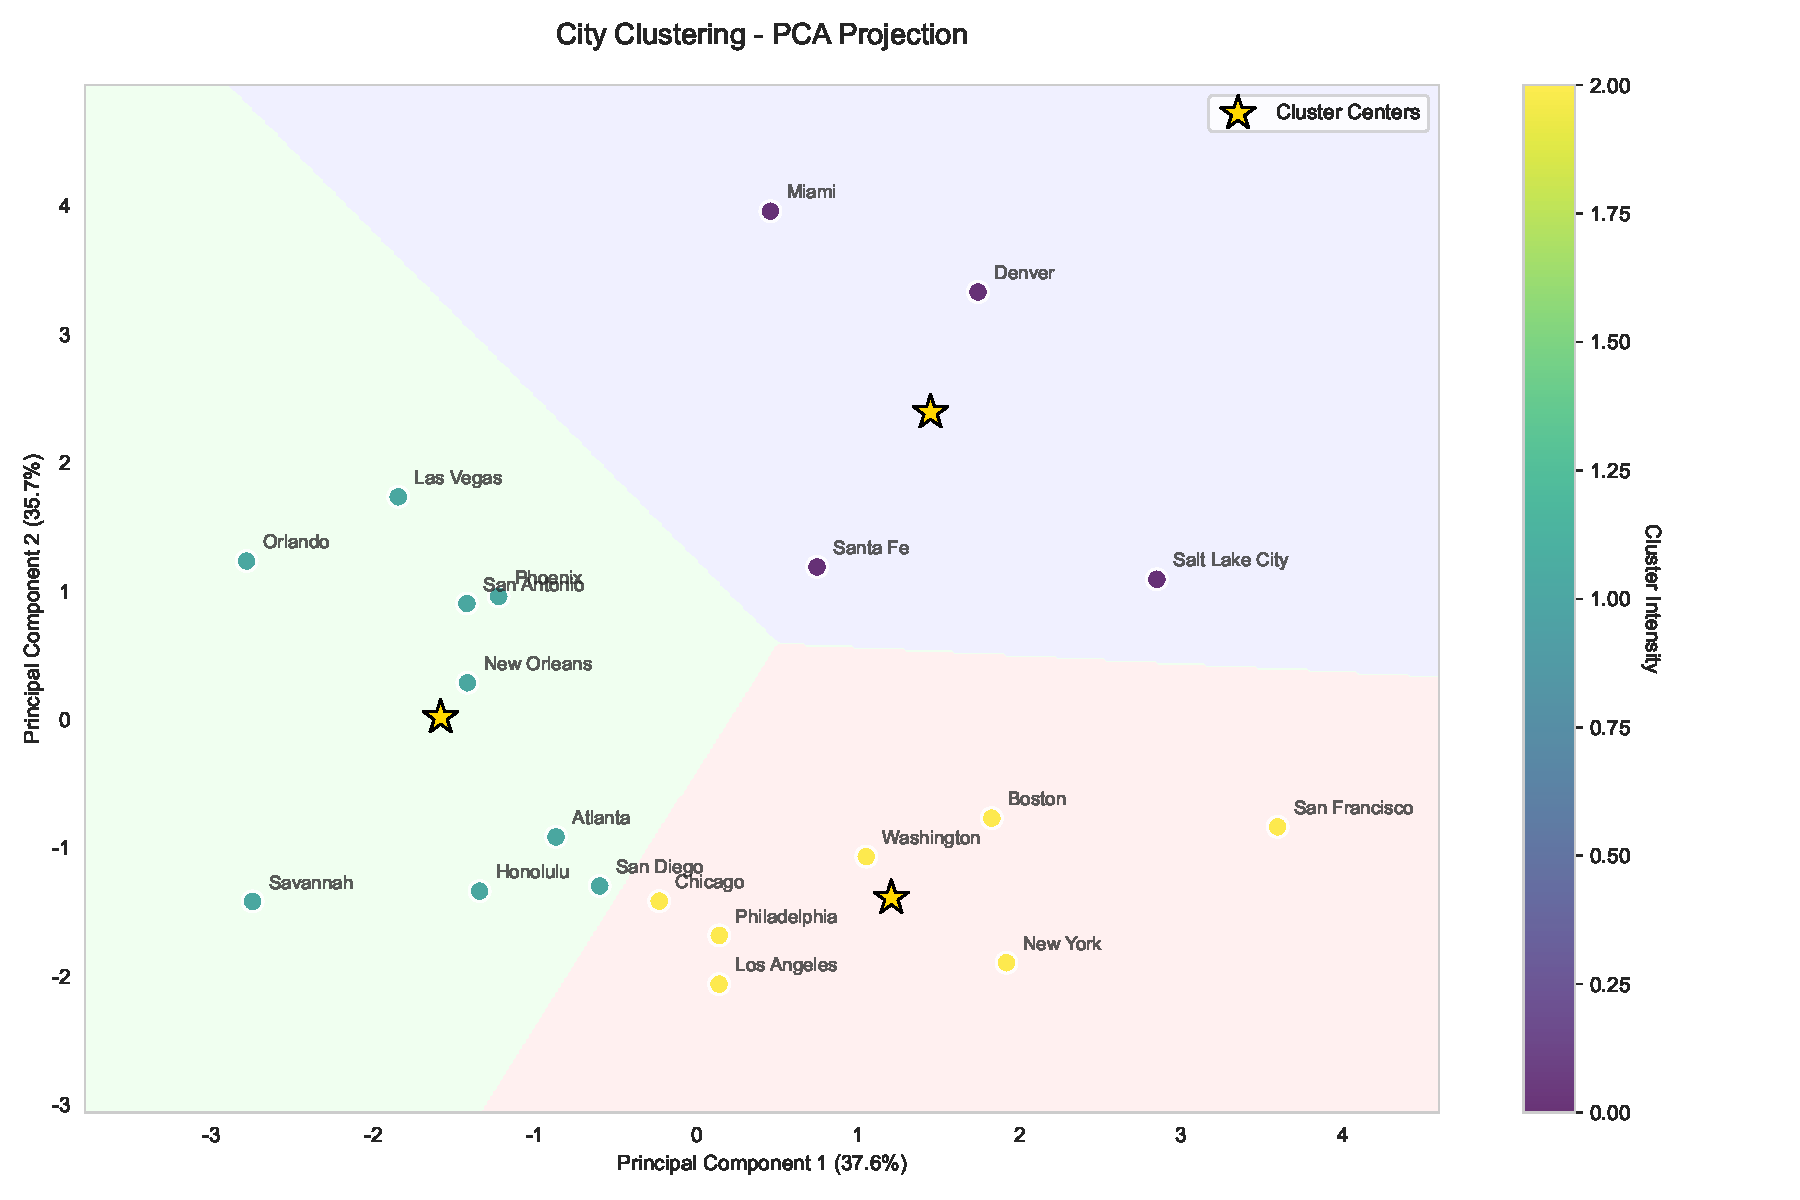
\includegraphics[width=\textwidth]{Kmeans.pdf}
  \caption{K-means cluster analysis results}
  \label{fig:kmeansresult}
\end{figure}
Through systematic observation of the clustering outcomes, we have formulated classification criteria for these cities as follows:\par
\subsubsection*{Cluster 1 (Santa Fe, Denver, Miami, Salt Lake City)}
\textbf{Medium Economic Scale, High Economic Growth → Prioritize Economic Development}
\begin{itemize}
    \item \textbf{High Economic Growth Potential}: Average GDP growth rates range between \textbf{0.10--0.14}, significantly higher than other clusters.
    \item \textbf{Rapid Income Growth}: Nominal income growth reaches \textbf{0.07--0.10}, closely aligning with GDP growth rates, indicating an active consumer market and effective translation of economic development into improved living standards.
    \item \textbf{Moderate Economic Scale}: Mean GDP ranges from \textbf{\$80.64 million to \$434 million}, reflecting an economy yet to reach saturation, with substantial untapped development potential.
\end{itemize}

\textbf{Development Recommendations:} \\
These cities exhibit robust economic momentum, high efficiency, and favorable returns on economic investments. Prioritize scaling investments (e.g., tourism infrastructure, commercial development) to unleash economic potential. Short-term goals should focus on maximizing growth, aligning with high tourist volume, high economic revenue, and large infrastructure investment solutions in the \textbf{Task1 model feasible set}.

\vspace{1em}
\hrule
\vspace{1em}

\subsubsection*{Cluster 2 (Atlanta, Honolulu, Las Vegas, etc.)}
\textbf{Low Economic Scale, Low Economic Growth → Prioritize Environmental Protection for Sustainable Development}
\begin{itemize}
    \item \textbf{Weak Economic Indicators}: Low mean GDP (\textbf{\$26.64 million--\$485 million}), with real income growth stagnation in some cities (e.g., Savannah: \textbf{real\_income\_calculate\_growth = -0.02}).
    \item \textbf{Unsustainable High Growth}: A few cities (e.g., Las Vegas) show GDP growth up to \textbf{0.15}, but nominal income growth remains at \textbf{0.07}, suggesting low industrial value-added, inefficient economic development, and environmental overdraft risks. Prioritize environmental conservation for high-quality sustainability.
\end{itemize}

\textbf{Development Recommendations:} \\
Address sluggish economic growth by enhancing industrial value-added, promoting green tourism (e.g. ecotourism, cultural heritage preservation), and balancing short-term gains with long-term sustainability. Align with \textbf{Task1 model solutions} emphasizing minimal environmental disruption, low greenhouse gas emissions, and high environmental protection investments.

\vspace{1em}
\hrule
\vspace{1em}

\subsubsection*{Cluster 3 (San Francisco, New York, Los Angeles, etc.)}
\textbf{High Economic Scale, Low Economic Growth → Balanced Development}
\begin{itemize}
    \item \textbf{Exceptionally Large Economic Scale}: Mean GDP exceeds \textbf{\$680 million} (e.g., New York: \textbf{\$20.1 billion}), nearing economic saturation.
    \item \textbf{Stable Growth}: GDP growth (\textbf{0.08--0.09}) and income growth (\textbf{0.05--0.06}) remain moderate, indicative of economic maturity.
    \item \textbf{High Income Levels}: Real income averages (e.g., San Francisco: \textbf{\$90,806}) significantly surpass other clusters, reflecting stable consumption structures.
\end{itemize}

\textbf{Development Recommendations:} \\
Optimize industrial structures (e.g., high-end cultural tourism, smart tourism) to enhance resource efficiency and achieve multidimensional equilibrium across economy, society, and environment. Implement \textbf{Task1 model solutions} balancing economic revenue with environmental protection, emphasizing high efficiency in cross-sectoral investments to drive advanced development.
\section{Task3: Writing Memorandum}
\subsection{Data Preconditions}
Since question 3 requires us to mention the forecast of data in the memorandum, and considering that the short-term forecast of Juneau is also an indispensable step in exploring the reasons for the city's sustainable tourism planning, we will make a forecast of the number of tourists from 2024 to 2030.
\subsubsection*{Method selection and model introduction}
\begin{itemize}
  \item Considering the data gaps in tourist statistics during 2020 and 2021 and the short-term forecasting objectives of this prediction task, through comparative analysis of various forecasting methodologies, we determined to employ the grey prediction method for subsequent data projections.
  \item Grey prediction analysis constitutes a small-sample forecasting approach tailored for incomplete information systems. Its core mechanism involves applying accumulation generation operations to fluctuating limited data, thereby mitigating stochastic disturbances and revealing latent continuous evolutionary patterns underlying the dataset. This method initially converts raw discrete data into a monotonically increasing sequence, constructs a dynamic model describing the system's holistic trends through exponential functions, and deduces future development trends by solving model parameters. Particularly applicable to short-term forecasting scenarios characterized by limited data volume, strong trend tendencies, yet significant fluctuations, the prediction process effectively balances computational efficiency with pattern recognition requirements.
\end{itemize}
\subsubsection*{Prediction process}
\begin{itemize}
  \item \textbf{Data preprocessing:} Considering that the grey prediction method requires continuous tourist data, and tourist data changed suddenly in 2020 and 2021 due to the COVID-19 pandemic, we only use data from 2010 to 2019 as the base volume.
  \item \textbf{Establishing the Grey Prediction Model GM(1,1):}
  \begin{itemize}
    \item \textbf{Original data sequence:} The collated tourist volume data is treated as the original data sequence \( X^{(0)} = \{x^{(0)}(1), x^{(0)}(2), \ldots, x^{(0)}(n)\} \).
    \item \textbf{First-order Accumulated Generating Operation:} Apply 1-AGO to the original data to generate a new sequence \( X^{(1)} = \{x^{(1)}(1), x^{(1)}(2), \ldots, x^{(1)}(n)\} \), where:
    $$x^{(1)}(k) = \sum_{i=1}^{k} x^{(0)}(i) $$  
    \item \textbf{Calculate cumulative sums:}\[
\begin{aligned}
x^{(1)}(1) &= 1532400, \\
x^{(1)}(2) &= 1532400 + 1556800 = 3089200, \\
x^{(1)}(3) &= 3089200 + 1586000 = 4675200, \\
&\vdots \\
x^{(1)}(12) &= 19833102 + 2760678 = 22593780.
\end{aligned}
\]
\item \textbf{Construct data matrix and vector:} Build the data matrix \( B \) and vector \( Y \) based on \( X^{(1)} \) for model parameter estimation:
\[
B = \begin{bmatrix}
-\frac{1}{2}\left(x^{(1)}(1) + x^{(1)}(2)\right) & 1 \\
-\frac{1}{2}\left(x^{(1)}(2) + x^{(1)}(3)\right) & 1 \\
\vdots & \vdots \\
-\frac{1}{2}\left(x^{(1)}(11) + x^{(1)}(12)\right) & 1
\end{bmatrix}, \quad 
Y = \begin{bmatrix}
x^{(0)}(2) \\
x^{(0)}(3) \\
\vdots \\
x^{(0)}(12)
\end{bmatrix}
\]
\item \textbf{Estimate model parameters:}  Use the least squares method to estimate the parameters \( a \) (development coefficient) and \( b \) (grey action quantity):
\[
\begin{bmatrix}
a \\
b
\end{bmatrix} = \left(B^T B\right)^{-1} B^T Y
\]
\item \textbf{Establish prediction model:} Construct the grey prediction model using parameters \( a \) and \( b \), and predict future values:
\[
\hat{x}^{(1)}(k) = \left(x^{(1)}(1) - \frac{b}{a}\right) e^{-a(k-1)} + \frac{b}{a}
\]

Obtain the predicted \( \hat{x}^{(0)}(k) \) through inverse accumulation:
\[
\hat{x}^{(0)}(k) = \hat{x}^{(1)}(k) - \hat{x}^{(1)}(k-1)
\]
  \end{itemize}
\end{itemize}
\subsubsection*{Prediction results}
Through the above system modeling and data analysis, we obtain a multi-dimensional prediction result for the development of tourism in Juno City: by inputting the tourist volume forecast data into the coupling model of carbon emissions, resident satisfaction and tourism revenue constructed in the early stage, the results show that the number of tourists will continue to rise, and it is expected to reach about 3 million in 2028; At the same time, tourism revenue will grow exponentially, with a significant increase of 117.1\% from the 2019 benchmark. It is worth noting that the expansion of tourism will have multiple negative effects – carbon emissions will increase dramatically, expected to reach 439,000 tonnes in 2028, and more challenging is the indicator of resident dissatisfaction, which will break through the 15\% threshold in 2026 and continue to rise, due to the dual pressure of overloaded infrastructure and deteriorating environmental quality. The model shows that without an effective regulatory mechanism, Juno will face risks such as degradation of ecosystem services, continuous deterioration of community relations, and collapse of urban carrying capacity, which highlights the urgency of tourism scale control and sustainable development strategy.
\begin{figure}
  \centering
  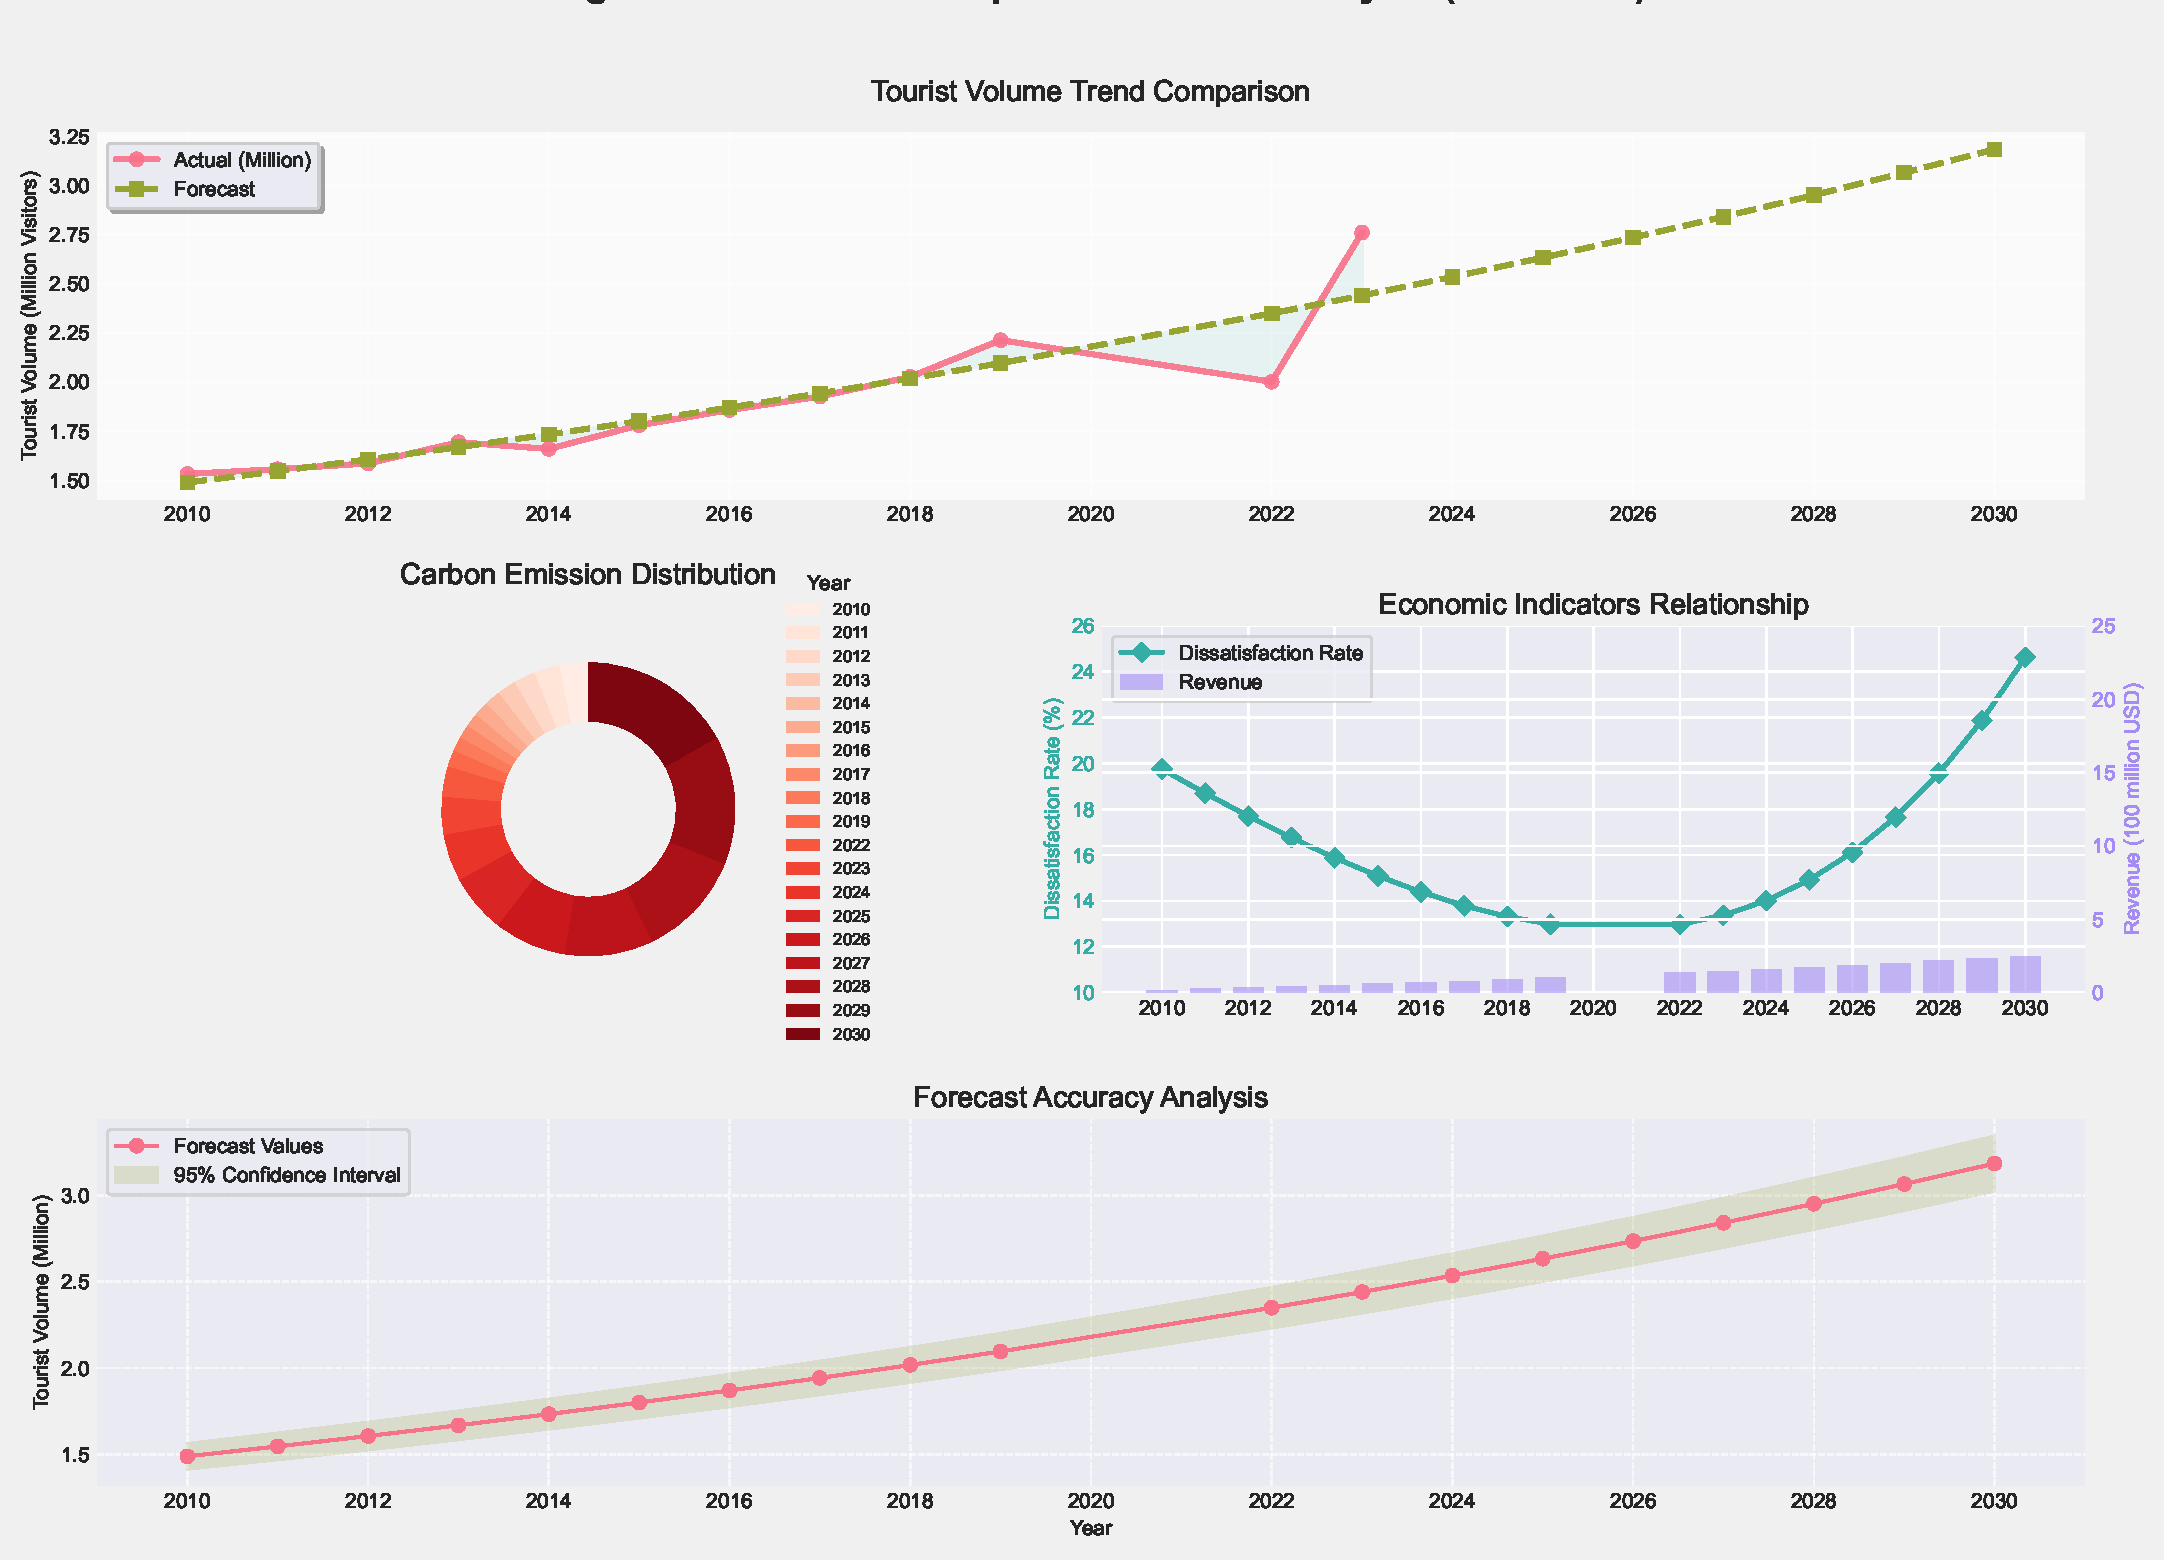
\includegraphics[width=\textwidth]{dataprediction.pdf}
  \caption{Data Preconditions from 2023 to 2030}
  \label{fig:predict}
\end{figure}

\section{Strength and Weakness}

\subsection{Strength}

\begin{itemize}
\item \textbf{Multi-objective optimization:} The model simultaneously optimizes economic benefit and carbon emissions, facilitating more comprehensive decision-making for achieving sustainable tourism development goals.
\item \textbf{Realistic constraints:} The four constraints, utilizing diverse models, cover factors such as visitor volume, traffic load, resident satisfaction, and carbon emissions, ensuring that the optimization results are highly applicable to real-world scenarios.
\item \textbf{Use of advanced algorithms:} The NSGA-III algorithm is employed, effectively identifying multiple Pareto optimal solutions and mitigating the one-sidedness that may arise from traditional single-objective optimization methods.
\end{itemize}

\subsection{Weakness}

\begin{itemize}
\item \textbf{Simplified assumptions:} The model's assumptions may be overly simplified, failing to comprehensively consider the influence of various social, economic, and cultural factors on visitor volume and carbon emissions.
\item \textbf{Overly conservative constraints:} Some constraints, such as traffic capacity and resident satisfaction, may be too stringent, limiting the flexibility of the model and restricting the breadth of the solution space.
\item \textbf{Dependence on data accuracy:} The model's results are highly dependent on the accuracy and timeliness of input data. Any discrepancies in the data may affect the reliability of the optimization outcomes.
\end{itemize}

\newpage
\newgeometry{left=0pt, right=0pt, top=0pt, bottom=0pt} % 临时去除页边距
\thispagestyle{empty} % 隐藏页眉页脚

\begin{figure}[p] % [p] 强制图片单独成页
  \centering
  \includegraphics[width=\paperwidth, height=\paperheight, keepaspectratio=false]{memo.pdf} % 覆盖整页(允许拉伸)
  \label{fig:fullpage}
\end{figure}

\restoregeometry % 恢复原始页边距
\begin{thebibliography}{99}
  \bibitem[Davies et al., 2024]{1}
  Davies, B., McNabb, R., Bendle, J. et al. 
  Accelerating glacier volume loss on Juneau Icefield driven by hypsometry and melt-accelerating feedbacks. 
  \textit{Nature Communications} \textbf{15}, 5099 (2024). 
  \url{https://doi.org/10.1038/s41467-024-49269-y}
  
  \bibitem[Wrangell Sentinel, 2023]{2}
  Wrangell Sentinel. 
  Tour operators will exceed visitor limit at Juneau's Mendenhall Glacier. 
  \emph{The oldest continuously published newspaper in Alaska}. 
  Retrieved from \url{https://www.wrangellsentinel.com/story/2023/07/19/news/tour-operators-will-exceed-visitor-limit-at-juneaus-mendenhall-glacier/12096.html}
  
  \bibitem[USDA, 2022]{3}
  United States Department of Agriculture. 
  Glacier visitor data: 443,000. 
  Retrieved from \url{https://www.govinfo.gov/content/pkg/GOVPUB-A13-PURL-gpo222163/pdf/GOVPUB-A13-PURL-gpo222163.pdf}
  
  \bibitem[City of Juneau, 2023]{4}
  City of Juneau. 
  Juneau Tourism Survey Report (2021-2023). 
  Retrieved from \url{https://juneau.org/wp-content/uploads/2021/12/Juneau-Tourism-Survey-Report-REV-12_1_21-1.pdf}
  
  \bibitem[JEDC, 2024]{5}
  Juneau Economic Development Council. 
  The Juneau \& Southeast Alaska Economic Indicators Reports (2012-2024). 
  Retrieved from \url{https://www.jedc.org/wp-content/uploads/2024/11/2024-JEDC-Juneau-SEAK-Economic-Indicators-and-Outlook-Report.pdf}
  
  \bibitem[City of Juneau, 2024]{6}
  City of Juneau. 
  Juneau Visitor Circulator Study Final Report. 
  Retrieved from \url{https://juneau.org/wp-content/uploads/2024/02/Juneau-Visitor-Circulator-Study-Final-Report-2024-1.pdf}
  
  \bibitem[EPA, n.d.]{7}
  U.S. Environmental Protection Agency. 
  EPA Greenhouse Gas Reporting Program: Aggregated County Data. 
  Retrieved from \url{https://www.epa.gov/ghgreporting}
  
  \bibitem[Anonymous, 2013]{8}
  The effect of government expenditure on the environment: An empirical investigation. 
  \emph{Ecological Economics}. 
  Retrieved from \url{https://doi.org/10.1016/j.ecolecon.2013.04.002}
  
  \bibitem[City of Juneau, 2020]{9}
  City of Juneau. 
  Administrative Guidelines: Hotel/Motel Room Tax Procedure 700. 
  Retrieved from \url{https://juneau.org/index.php?gf-download=2020%2F01%2F700_Hotel-Motel_Tax_Procedures_2020.pdf}
  
  \bibitem[NAHB, n.d.]{10}
  National Association of Home Builders. 
  Housing Economics: Residential Building Cost and Income Ratio. 
  Retrieved from \url{https://www.nahb.org/news-and-economics/housing-economics}
  
  \bibitem[Alaska CRF, n.d.]{11}
  Alaska Carbon Reduction Fund. 
  Tax implications for carbon emissions. 
  Retrieved from \url{https://akcarbonreduction.org/}
  \end{thebibliography}

% \begin{thebibliography}{99}
%   \bibitem{abc} D.~E. KNUTH   The \TeX{}book  the American
%   Mathematical Society and Addison-Wesley
%   Publishing Company , 1984-1986.
%   \bibitem{2}Lamport, Leslie,  \LaTeX{}: `` A Document Preparation System '',
%   Addison-Wesley Publishing Company, 1986.
%   \bibitem{3}\url{https://www.latexstudio.net/}
%   \end{thebibliography}

\newpage

% \begin{appendices}

% \section{First appendix}

% In addition, your report must include a letter to the Chief Financial Officer (CFO) of the Goodgrant Foundation, Mr. Alpha Chiang, that describes the optimal investment strategy, your modeling approach and major results, and a brief discussion of your proposed concept of a return-on-investment (ROI). This letter should be no more than two pages in length.

% Here are simulation programmes we used in our model as follow.\\

% \textbf{\textcolor[rgb]{0.98,0.00,0.00}{Input matlab source:}}
% \lstinputlisting[language=Matlab]{./code/mcmthesis-matlab1.m}

% \section{Second appendix}

% some more text \textcolor[rgb]{0.98,0.00,0.00}{\textbf{Input C++ source:}}
% \lstinputlisting[language=C++]{./code/mcmthesis-sudoku.cpp}

% \end{appendices}

\newpage
\newcounter{lastpage}
\setcounter{lastpage}{\value{page}}
\thispagestyle{empty} 

\section*{Report on Use of AI}

\begin{enumerate}
\item Open AI Chatgt4o 
\begin{description}
\item[Query1:] What are some cities in the United States with a developed tourism industry? 
\item[Output:] Here’s the translation of the provided text:
Tourist cities in the United States are typically those with rich culture, historical landmarks, natural beauty, and modern facilities. Here are some famous tourist cities:
New York City
As the largest and most diverse city in the U.S., New York is home to countless iconic attractions, including the Statue of Liberty, Times Square, Central Park, museums (such as the Metropolitan Museum of Art and the Museum of Modern Art), and Broadway.
\begin{itemize}
  \item \textbf{Los Angeles}
  Los Angeles is the birthplace of Hollywood, with popular tourist attractions such as the Hollywood Walk of Fame, Universal Studios, Griffith Observatory, and beautiful beaches (like Santa Monica and Venice Beach).
  Las Vegas
  Known for its world-class casinos, nightlife, luxury hotels, and entertainment shows, Las Vegas offers unparalleled nighttime excitement and top-tier performances.
  \item \textbf{San Francisco}
  San Francisco is famous for the Golden Gate Bridge, Fisherman’s Wharf, Alcatraz Island, and its hilly streets. The city offers many cultural activities and unique scenic spots.
  \item \textbf{Washington, D.C.}
  As the capital of the United States, Washington, D.C. has a rich historical heritage, including the Capitol Building, the White House, the Lincoln Memorial, and the Smithsonian Institution museums.
  \item \textbf{Miami}
  Known for its tropical climate, white sand beaches, Latin culture, and vibrant nightlife, Miami is also a popular vacation destination in the U.S.
  \item \textbf{Chicago}
  Chicago has a deep cultural background, with tourists visiting Millennium Park, the Art Institute of Chicago, Navy Pier, and its famous skyscrapers.
  \item \textbf{Boston}
  Boston is one of the most historically significant cities in the U.S., with many historical sites such as the Freedom Trail, the Boston Tea Party Ships and Museum.
  These cities have become hotspots for tourism in the U.S. due to their unique culture, history, entertainment, and natural beauty. Do you have a preference for any of these cities, or would you like to learn more about a specific one?
\end{itemize}

\end{description}
\item Open AI Chatgt4o 
\begin{description}
\item[Query1:] The area of Juneau, Alaska, USA is how much? 
\item[Output:] Juneau is the capital of Alaska, USA. Its total area is 3,255.0 square miles (8,430.4 square kilometers), which includes 2,715.7 square miles (7,036.1 square kilometers) of land and 539.3 square miles (1,394.3 square kilometers) of water.
\end{description}
\item Open AI Chatgt4o 
\begin{description}
\item[Query1:] "I am now going to perform cluster analysis on some famous tourist cities in the United States. How many indicators do you think are needed?" 
\item[Output:] You can choose a suitable combination of these indicators, focusing on those that best reflect the tourism characteristics of the cities. If you're doing a basic cluster analysis, I recommend using the following key indicators as a foundation:
\begin{itemize}
  \item \textbf{Population Size}
  \item \textbf{Tourism Revenue}
  \item \textbf{Number of Tourist Attractions}
  \item \textbf{Annual Tourist Arrival Numbers}
  \item \textbf{Transportation Accessibility} (such as the number of airports)
  \item \textbf{Safety Index}
\end{itemize}
These indicators cover aspects such as city size, tourism appeal, and accommodation capacity, helping you classify and analyze cities from various perspectives. If you have time and data, you can also include more dimensions (such as price level and climate) to further refine the clustering results.
What data are you planning to use for the analysis? Feel free to share some specific tourist cities and data, and I can help you design the cluster model more concretely.
\end{description}
\item Open AI Chatgt4o 
\begin{description}
\item[Query1:] The Relationship Between Carbon Footprint and Carbon Emissions
\item[Output:] The Relationship Between Carbon Footprint and Carbon Emissions
Carbon Emissions refer to the direct release of carbon dioxide (CO2) and other greenhouse gases (GHGs) into the atmosphere, primarily from human activities such as burning fossil fuels, industrial processes, and deforestation. These emissions contribute directly to global warming and climate change.
Carbon Footprint, on the other hand, is a broader measure. It refers to the total amount of CO2 and other GHG emissions that are directly and indirectly associated with a particular activity, product, individual, organization, or nation. This includes not only the carbon emissions from energy use (e.g., electricity, fuel consumption) but also emissions from the entire lifecycle of goods and services—such as transportation, manufacturing, and waste generation.
Relationship:
\begin{itemize}
  \item Carbon emissions are a key component of a carbon footprint. The carbon footprint is essentially the sum of all carbon emissions from the production, consumption, and disposal processes related to a specific activity or entity.
  \item	For example, if an individual drives a car, the direct carbon emissions from fuel combustion contribute to their carbon footprint. Additionally, the carbon footprint would include the emissions generated in the production of the car, the extraction of raw materials, and the disposal of the car at the end of its life.
  \item	Thus, carbon emissions are a direct measurement of GHG output, while a carbon footprint encompasses the entire lifecycle of activities or products and includes both direct and indirect emissions.
  \end{itemize}
  In summary, carbon emissions contribute to the carbon footprint, but the carbon footprint includes a wider scope, capturing both direct and indirect emissions across the supply chain.
\end{description}
\end{enumerate}

% 重置页码
\clearpage
\setcounter{page}{\value{lastpage}}

\end{document}

